\documentclass[
%draft,           %use this for fast draft compilation with additional overfull boxes hint bars (also affects graphicx)
a4paper,          %A4 paper size
11pt,             %well readable for A4 printing
cleardoubleempty, %nice left plain pages before chapters
%chapterprefix,    %chapter X prefix before chapters
%appendixprefix,   %appendix X prefix before appendices
headsepline,      %lines in header
headtopline,      %lines in header
footbotline,      %lines in footer
footsepline,      %lines in footer
plainfootbotline, %lines in footer for scrplain page style
plainfootsepline, %lines in footer for srcplain page style
ilines,
DIV18,            %adjust this value for more/less text on pages
BCOR5mm]{scrbook}
\usepackage[]{scrpage2} %%% koma script for nice layout
\usepackage[english, ngerman]{babel}   %%% an english thesis usually has a german synopsis

% \usepackage{scrltx}
%\usepackage{layout}  %%% may be needed if i steal some more code from other thesises
\usepackage{exscale} %%% for proportional sum and integral signs

\usepackage[
numbers, 
square, 
comma, 
sort&compress]{natbib} % Order the citations

%\usepackage{struktex} %%% create structograms
\usepackage{booktabs} %%% scientific publication style tables
\usepackage{empheq}   %%% for boxed equations and alike
\usepackage{xcolor,colortbl}  %%% for colored text, formulae and tables
\usepackage{amsmath}  %%% math symbols needed
\usepackage{amsfonts} %%% math fonts needed
\usepackage{amssymb}  %%% maths symbols needed 
\usepackage{amsthm}   %%% theorem environments
\usepackage{dsfont}   %%% for blackboard numbers and characters 
%\usepackage{mathdots/mathdots}

\usepackage{fancybox} %%% more types of boxes 

\usepackage{graphicx}       %%% CUSTOMIZATION: include all pictures
%\usepackage[draft]{graphicx} %%% choose draft option for faster compiling without pictures
\graphicspath{{Figures/}}      %%% all pictures will reside there and in subdirs

%\usepackage[rlft]{floatflt} %%% allows text wraping of floating figures 
\usepackage{float}      %%% define custom float environments
%\usepackage[plainpages=false,colorlinks]{hyperref} %%% CUSTOMIZATION use this package for the final compilation run for online publication, includes hyperlinks for sections/eqs/etc.
\usepackage[]{hyperref} %%% CUSTOMIZATION use this package for the final compilation run for online publication, includes hyperlinks for sections/eqs/etc.
%\usepackage{subfigure}  %%% nice captioning and referencing of subfigures
\usepackage{subcaption}
\usepackage{caption}    %%% (load after subfigure package) nicer layout for figure captions
%\usepackage[notref,notcite]{showkeys} %%% show labels for equations and pictures on the margin(intended for development state) 


%%%%%%%%%%%%%%%%%%%%%%%%%%%%%%%%%%%%%%%%%%%%%%%%%%
%%% Selection of the fonts!!
\usepackage[T1]{fontenc}
\usepackage{helvet}
%%%%%%%%%%%%%%%%%%%%%%%%%%%%%%%%%%%%%%%%%%%%%%%%%%

%ANNES PACKAGES
\usepackage{siunitx}
\usepackage[above]{placeins}
\usepackage{stfloats}
\usepackage[utf8]{inputenc}
\usepackage[T1]{fontenc}
\usepackage[italic]{hepnames}
\usepackage[final]{pdfpages} %set to "final" in the end to show the pdf page
\usepackage{multirow}
\usepackage{verbatim}
\usepackage{rotating}
\usepackage{array} 
\usepackage{pifont}
\usepackage{setspace}
\usepackage{textcomp}
\usepackage{siunitx}
%\usepackage[]{units}
\usepackage{tabularx}
\setcounter{tocdepth}{3}
\setcounter{secnumdepth}{3}

\usepackage{todonotes} %Added by Phill so that todo lists can be added
\setlength{\marginparwidth}{2cm} %This stops the todo notes from overflowing the page

\newcommand{\myparagraph}[1]{\thesubsubsection\ \alph{paragraph}{#1}\mbox{}\\}
\newcommand{\redcomment}[1]{\ding{110}\ding{43}\textcolor{red}{#1}}

\newcommand{\slic}{\textsc{SLIC}\xspace}
\newcommand{\gdml}{\textsc{GDML}\xspace}
\newcommand{\xml}{\textsc{XML}\xspace}
\newcommand{\lcdd}{\textsc{LCDD}\xspace}
\newcommand{\lcio}{\textsc{LCIO}\xspace}
\newcommand{\ilcsoft}{\textsc{ILCSoft}\xspace}
\newcommand{\marlin}{\textsc{Marlin}\xspace}
\newcommand{\Root}{\textsc{ROOT}\xspace}
\newcommand{\Cplusplus}{\texttt{C++}\xspace}
\newcommand{\geant}{\textsc{Geant4}\xspace}
\newcommand{\bdsim}{\textsc{BDSIM}\xspace}
\newcommand{\mucarlo}{\textsc{MUCARLO}\xspace}
\newcommand{\fluka}{\textsc{FLUKA}\xspace}
\newcommand{\flair}{\textsc{FLAIR}\xspace}
\newcommand{\degree}{\ensuremath{^\circ}}
\newcommand{\electron}{e$^-$\xspace}
\newcommand{\positron}{e$^+$\xspace}
\newcommand{\lumi}{$\mathcal{L}$\xspace}

%------Definition for column color in table
\definecolor{Gray}{gray}{0.9}
\newcolumntype{g}{>{\columncolor{Gray}}r}
%-----------------------------------------

\ExplSyntaxOn

\makeatletter
\NewDocumentCommand{\multicitep}{m}
 {
  \NAT@open
  \mjb_multicitep:n { #1 }
  \NAT@close
 }
\makeatother

\seq_new:N \l_mjb_multicite_in_seq
\seq_new:N \l_mjb_multicite_out_seq
\seq_new:N \l_mjb_cite_seq

\cs_new_protected:Npn \mjb_multicitep:n #1
 {
  \seq_set_split:Nnn \l_mjb_multicite_in_seq { ; } { #1 }
  \seq_clear:N \l_mjb_multicite_out_seq
  \seq_map_inline:Nn \l_mjb_multicite_in_seq
   {
    \mjb_cite_process:n { ##1 }
   }
  \seq_use:Nn \l_mjb_multicite_out_seq { ;~ }
 }

\cs_new_protected:Npn \mjb_cite_process:n #1
 {
  \seq_set_split:Nnn \l_mjb_cite_seq { , } { #1 }
  \int_compare:nTF { \seq_count:N \l_mjb_cite_seq == 1 }
   {
    \seq_put_right:Nn \l_mjb_multicite_out_seq
     { \cite{#1}}
   }
   {
    \seq_put_right:Nx \l_mjb_multicite_out_seq
     {
      \exp_not:N \cite{\seq_item:Nn \l_mjb_cite_seq { 1 }},~
      \seq_item:Nn \l_mjb_cite_seq { 2 }
     }
   }
 }
\ExplSyntaxOff

%SIMONS COMMANDS FOR TITLEPAGE
\usepackage{tikz}
\def\changemargin#1#2{\list{}{\rightmargin#2\leftmargin#1}\item[]}
\let\endchangemargin=\endlist 
\usepackage[absolute]{textpos}
\newcommand{\changefont}[3]{
\fontfamily{#1}\fontseries{#2}\fontshape{#3}\selectfont}

\newcommand{\myname}{Anne Schütz}
\newcommand{\mytitle}{Optimizing the design of the Final-Focus Region\\for the International Linear Collider}
\newcommand{\myinstitute}{Institute of Experimental Nuclear Physics (IEKP)}
\newcommand{\mydepartment}{Department of Physics}
\newcommand{\myuniversity}{Karlsruhe Institute of Technology}

\newcommand{\reviewerone}{Prof. Dr. Günter Quast (IEKP)}
\newcommand{\reviewertwo}{Prof. Dr. Eckhard Elsen (DESY)}
\newcommand{\advisor}{Dr. Marcel Stanitzki (DESY)}


\newcommand{\timestart}{April 01, 2015}
\newcommand{\timeend}{March 31, 2018}
%\newcommand{\submissiontime}{DD. MM. 20XX}

%%%%%%%%%%%%%%%%%%%%%%%%%%%%%%%%%%%%%%%%%%%%%%%%%%
%%% user defined abbreviations/commands/macros/layout commands

%%%%%%%%%%%%%%%%%%%%%%%%%%%%%%%%%%%%%%%%%%%%%%%%%%
%%%%%%%%%%%%%%%%%%%%%%%%%%%%%%%%%%%%%%%%%%%%%%%%%%
%%%
%%% here all macros and definitions concerning layout will be gathered
%%%
%%%%%%%%%%%%%%%%%%%%%%%%%%%%%%%%%%%%%%%%%%%%%%%%%%
%%%%%%%%%%%%%%%%%%%%%%%%%%%%%%%%%%%%%%%%%%%%%%%%%%

%%%%%%%%%%%%%%%%%%%%%%%%%%%%%%%%%%%%%%%%%%%%%%%%%%
%%% description label font
%%%%%%%%%%%%%%%%%%%%%%%%%%%%%%%%%%%%%%%%%%%%%%%%%%
%%% When using helvetic as font, the description labels become to
%%% large, so let's use the standard text font and make it bold (which
%%% i like better anyways...)
\setkomafont{descriptionlabel}{\normalfont\bfseries}

%%%%%%%%%%%%%%%%%%%%%%%%%%%%%%%%%%%%%%%%%%%%%%%%%%
%%% hyperlinks and bookmarks menu for online reading
%%%%%%%%%%%%%%%%%%%%%%%%%%%%%%%%%%%%%%%%%%%%%%%%%%
\hypersetup{bookmarksopen=true,
bookmarksnumbered=true}

%%% general unit is 1 cm
%\setlength{\unitlength}{1cm}

%%%%%%%%%%%%%%%%%%%%%%%%%%%%%%%%%%%%%%%%%%%%%%%%%%
%%% the abstract before each chapter telling the reader
%%% what will be described here
%%%%%%%%%%%%%%%%%%%%%%%%%%%%%%%%%%%%%%%%%%%%%%%%%%
\newenvironment{chapterabstract}{\itshape}{}

%%%%%%%%%%%%%%%%%%%%%%%%%%%%%%%%%%%%%%%%%%%%%%%%%%
%%% the source file of an image
%%%%%%%%%%%%%%%%%%%%%%%%%%%%%%%%%%%%%%%%%%%%%%%%%%
\newcommand{\code}[1]{\texttt{\small{#1}}}
\newcommand{\filename}[1]{\texttt{#1}}
\newcommand{\sourcename}[1]{{\footnotesize Source:\\\filename{#1}}}

\newcommand{\packagename}[1]{{\sffamily #1}}
%%%%%%%%%%%%%%%%%%%%%%%%%%%%%%%%%%%%%%%%%%%%%%%%%%
%%% shortcuts to refer to environments and sections
%%%%%%%%%%%%%%%%%%%%%%%%%%%%%%%%%%%%%%%%%%%%%%%%%%
%\newcommand{\citep}[2][]{\mbox{Refs.~\cite[#2]{#1}}}
\newcommand{\pref}[1]{\mbox{page \pageref{#1}}}
\newcommand{\Eqref}[1]{\mbox{Eq.~(\ref{#1})}}
\newcommand{\eqrefp}[1]{\mbox{Eqs.~(\ref{#1})}}
\newcommand{\tabref}[1]{\mbox{Tab.~\ref{#1}}}
\newcommand{\tabrefp}[1]{\mbox{Tabs.~\ref{#1}}}
\newcommand{\figref}[1]{\mbox{Fig.~\ref{#1}}}
\newcommand{\figrefp}[1]{\mbox{Figs.~\ref{#1}}}
\newcommand{\secref}[1]{\mbox{Sec.~\ref{#1}}}
\newcommand{\secrefp}[1]{\mbox{Secs.~\ref{#1}}}
\newcommand{\chapref}[1]{\mbox{Chap.~\ref{#1}}}
\newcommand{\chaprefp}[1]{\mbox{Chaps.~\ref{#1}}}

%%%%%%%%%%%%%%%%%%%%%%%%%%%%%%%%%%%%%%%%%%%%%%%%%%
%%% layout for caption and captionlabels
%%%%%%%%%%%%%%%%%%%%%%%%%%%%%%%%%%%%%%%%%%%%%%%%%%
\renewcommand{\captionfont}{\itshape}
\renewcommand{\captionlabelfont}{\bfseries \upshape}
\setlength{\captionmargin}{10pt}

%%%%%%%%%%%%%%%%%%%%%%%%%%%%%%%%%%%%%%%%%%%%%%%%%%
%%% create boxed formulas within a math environment
%%% carriage return is allowed in the source
%%% (this is not the case when using the AMS command \boxed)
%%%%%%%%%%%%%%%%%%%%%%%%%%%%%%%%%%%%%%%%%%%%%%%%%%
\newcommand{\mathbox}[1]{
    \fbox{ $ \displaystyle #1 $ }
}


%%%%%%%%%%%%%%%%%%%%%%%%%%%%%%%%%%%%%%%%%%%%%%%%%%
%%% a single named theorem environment for the
%%% bloch-floquet theorem
%%%%%%%%%%%%%%%%%%%%%%%%%%%%%%%%%%%%%%%%%%%%%%%%%%
\newtheorem*{BlochFloquetTheorem}{Bloch-Floquet Theorem}
\newtheorem{theorem}{Theorem}


%%%%%%%%%%%%%%%%%%%%%%%%%%%%%%%%%%%%%%%%%%%%%%%%%%
%%% set the style of the bibliography
%%%%%%%%%%%%%%%%%%%%%%%%%%%%%%%%%%%%%%%%%%%%%%%%%%
%\bibliographystyle{unsrtnat}

%%%%%%%%%%%%%%%%%%%%%%%%%%%%%%%%%%%%%%%%%%%%%%%%%%
%%% a general purpose width, set where needed and
%%% helps typesetting mainly math equations where
%%% equal box sizes are needed
%%%%%%%%%%%%%%%%%%%%%%%%%%%%%%%%%%%%%%%%%%%%%%%%%%
\newlength{\auxwidth} 

%%%%%%%%%%%%%%%%%%%%%%%%%%%%%%%%%%%%%%%%%%%%%%%%%%
%%% width for mode pictures,
%%% which will be set side by side. this width is
%%% set when needed
%%%%%%%%%%%%%%%%%%%%%%%%%%%%%%%%%%%%%%%%%%%%%%%%%%
\newlength{\modewidth} 

%%%%%%%%%%%%%%%%%%%%%%%%%%%%%%%%%%%%%%%%%%%%%%%%%%
%%% separator line widths
%%%%%%%%%%%%%%%%%%%%%%%%%%%%%%%%%%%%%%%%%%%%%%%%%%
\setheadtopline{2pt}
\setheadsepline{0.5pt}
\setfootsepline{0.5pt}
\setfootbotline{2pt}

\delimitershortfall=-2pt

%%%%%%%%%%%%%%%%%%%%%%%%%%%%%%%%%%%%%%%%%%%%%%%%%%
%%% width for one, two, three, four plots per line
%%%%%%%%%%%%%%%%%%%%%%%%%%%%%%%%%%%%%%%%%%%%%%%%%%
\newlength{\plotwidthOne} 
\setlength{\plotwidthOne}{0.975\textwidth} 
\newlength{\plotwidthTwo} 
\setlength{\plotwidthTwo}{0.477\textwidth} 
\newlength{\plotwidthThree} 
\setlength{\plotwidthThree}{0.31\textwidth} 
\newlength{\plotwidthThreeTwo} 
\setlength{\plotwidthThreeTwo}{0.642\textwidth} 
\newlength{\plotwidthThreeOne} 
\setlength{\plotwidthThreeOne}{0.31\textwidth} 
\newlength{\plotwidthFour} 
\setlength{\plotwidthFour}{0.227\textwidth} 

\newcommand{\includesingleplot}[1]{
  \parbox{\singleplotwidth}{
    \includegraphics[width=\plotwidthTwo]{#1}\\
    \sourcename{#1.agr}
  }
}
\newcommand{\includedoubleplot}[1]{
  \parbox{\doubleplotwidth}{
    \includegraphics[width=\plotwidthOne]{#1}\\
    \sourcename{#1.agr}
  }
}
\newcommand{\includeannotatedplot}[3]{
  \parbox{#1}{
    \centering    
    \includegraphics[width=#1]{#2}\\
    #3
  }
}

%%% define a new floating environment used for tables and figures side by side
\newfloat{hybridfloat}{ht}{hybridfloat}


%%%%%%%%%%%%%%%%%%%%%%%%%%%%%%%%%%%%%%%%%%%%%%%%%%%%%%%%%%%%
%%%%%%%%%%%%%%%%%%%%%%%%%%%%%%%%%%%%%%%%%%%%%%%%%%%%%%%%%%%%
%%%%%%%                            %%%%%%%%%%%%%%%%%%%%%%%%%
%%%%%   color definitions            %%%%%%%%%%%%%%%%%%%%%%%
%%%%%%                             %%%%%%%%%%%%%%%%%%%%%%%%%
%%%%%%%%%%%%%%%%%%%%%%%%%%%%%%%%%%%%%%%%%%%%%%%%%%%%%%%%%%%%
%%%%%%%%%%%%%%%%%%%%%%%%%%%%%%%%%%%%%%%%%%%%%%%%%%%%%%%%%%%%
\definecolor{greenyellow}   {cmyk}{0.15, 0   , 0.69, 0   }
\definecolor{yellow}        {cmyk}{0   , 0   , 1   , 0   }
\definecolor{goldenrod}     {cmyk}{0   , 0.10, 0.84, 0   }
\definecolor{dandelion}     {cmyk}{0   , 0.29, 0.84, 0   }
\definecolor{apricot}       {cmyk}{0   , 0.32, 0.52, 0   }
\definecolor{peach}         {cmyk}{0   , 0.50, 0.70, 0   }
\definecolor{melon}         {cmyk}{0   , 0.46, 0.50, 0   }
\definecolor{yelloworange}  {cmyk}{0   , 0.42, 1   , 0   }
\definecolor{orange}        {cmyk}{0   , 0.61, 0.87, 0   }
\definecolor{burntorange}   {cmyk}{0   , 0.51, 1   , 0   }
\definecolor{bittersweet}   {cmyk}{0   , 0.75, 1   , 0.24}
\definecolor{redorange}     {cmyk}{0   , 0.77, 0.87, 0   }
\definecolor{mahogany}      {cmyk}{0   , 0.85, 0.87, 0.35}
\definecolor{maroon}        {cmyk}{0   , 0.87, 0.68, 0.32}
\definecolor{brickred}      {cmyk}{0   , 0.89, 0.94, 0.28}
\definecolor{red}           {cmyk}{0   , 1   , 1   , 0   }
\definecolor{orangered}     {cmyk}{0   , 1   , 0.50, 0   }
\definecolor{rubinered}     {cmyk}{0   , 1   , 0.13, 0   }
\definecolor{wildstrawberry}{cmyk}{0   , 0.96, 0.39, 0   }
\definecolor{salmon}        {cmyk}{0   , 0.53, 0.38, 0   }
\definecolor{carnationpink} {cmyk}{0   , 0.63, 0   , 0   }
\definecolor{magenta}       {cmyk}{0   , 1   , 0   , 0   }
\definecolor{violetred}     {cmyk}{0   , 0.81, 0   , 0   }
\definecolor{rhodamine}     {cmyk}{0   , 0.82, 0   , 0   }
\definecolor{mulberry}      {cmyk}{0.34, 0.90, 0   , 0.02}
\definecolor{redviolet}     {cmyk}{0.07, 0.90, 0   , 0.34}
\definecolor{fuchsia}       {cmyk}{0.47, 0.91, 0   , 0.08}
\definecolor{lavender}      {cmyk}{0   , 0.48, 0   , 0   }
\definecolor{thistle}       {cmyk}{0.12, 0.59, 0   , 0   }
\definecolor{orchid}        {cmyk}{0.32, 0.64, 0   , 0   }
\definecolor{darkorchid}    {cmyk}{0.40, 0.80, 0.20, 0   }
\definecolor{purple}        {cmyk}{0.45, 0.86, 0   , 0   }
\definecolor{plum}          {cmyk}{0.50, 1   , 0   , 0   }
\definecolor{violet}        {cmyk}{0.79, 0.88, 0   , 0   }
\definecolor{royalpurple}   {cmyk}{0.75, 0.90, 0   , 0   }
\definecolor{blueviolet}    {cmyk}{0.86, 0.91, 0   , 0.04}
\definecolor{periwinkle}    {cmyk}{0.57, 0.55, 0   , 0   }
\xdefinecolor{cadetblue}     {cmyk}{0.62, 0.57, 0.23, 0   }
\xdefinecolor{cornflowerblue}{cmyk}{0.65, 0.13, 0   , 0   }
\xdefinecolor{midnightblue}  {cmyk}{0.98, 0.13, 0   , 0.43}
\xdefinecolor{navyblue}      {cmyk}{0.94, 0.54, 0   , 0   }
\xdefinecolor{royalblue}     {cmyk}{1   , 0.50, 0   , 0   }
\definecolor{blue}          {cmyk}{1   , 1   , 0   , 0   }
\xdefinecolor{darkblue}     {cmyk}{1   , 1   , 0   , 0.5 }
\definecolor{cerulean}      {cmyk}{0.94, 0.11, 0   , 0   }
\definecolor{cyan}          {cmyk}{1   , 0   , 0   , 0   }
\definecolor{processblue}   {cmyk}{0.96, 0   , 0   , 0   }
\definecolor{skyblue}       {cmyk}{0.62, 0   , 0.12, 0   }
\definecolor{turquoise}     {cmyk}{0.85, 0   , 0.20, 0   }
\definecolor{tealblue}      {cmyk}{0.86, 0   , 0.34, 0.02}
\definecolor{aquamarine}    {cmyk}{0.82, 0   , 0.30, 0   }
\definecolor{bluegreen}     {cmyk}{0.85, 0   , 0.33, 0   }
\definecolor{emerald}       {cmyk}{1   , 0   , 0.50, 0   }
\definecolor{junglegreen}   {cmyk}{0.99, 0   , 0.52, 0   }
\definecolor{seagreen}      {cmyk}{0.69, 0   , 0.50, 0   }
\definecolor{green}         {cmyk}{1   , 0   , 1   , 0   }
\definecolor{forestgreen}   {cmyk}{0.91, 0   , 0.88, 0.12}
\definecolor{pinegreen}     {cmyk}{0.92, 0   , 0.59, 0.25}
\definecolor{limegreen}     {cmyk}{0.50, 0   , 1   , 0   }
\definecolor{yellowgreen}   {cmyk}{0.44, 0   , 0.74, 0   }
\definecolor{springgreen}   {cmyk}{0.26, 0   , 0.76, 0   }
\definecolor{olivegreen}    {cmyk}{0.64, 0   , 0.95, 0.40}
\definecolor{rawsienna}     {cmyk}{0   , 0.72, 1   , 0.45}
\definecolor{sepia}         {cmyk}{0   , 0.83, 1   , 0.70}
\definecolor{brown}         {cmyk}{0   , 0.81, 1   , 0.60}
\definecolor{tan}           {cmyk}{0.14, 0.42, 0.56, 0   }
\definecolor{gray}          {cmyk}{0   , 0   , 0   , 0.50}
\definecolor{black}         {cmyk}{0   , 0   , 0   , 1   }
\definecolor{white}         {cmyk}{0   , 0   , 0   , 0   } 
\definecolor{darkgray}      {cmyk}{0   , 0   , 0   , 0.75}


%%%%%%%%%%%%%%%%%%%%%%%%%%%%%%%%%%%%%%%%%%%%%%%%%%%%%%%%%%%%
%%%%%%%%%%%%%%%%%%%%%%%%%%%%%%%%%%%%%%%%%%%%%%%%%%%%%%%%%%%%
%%%%%%%                            %%%%%%%%%%%%%%%%%%%%%%%%%
%%%%%   chapter headings             %%%%%%%%%%%%%%%%%%%%%%%
%%%%%%                             %%%%%%%%%%%%%%%%%%%%%%%%%
%%%%%%%%%%%%%%%%%%%%%%%%%%%%%%%%%%%%%%%%%%%%%%%%%%%%%%%%%%%%
%%%%%%%%%%%%%%%%%%%%%%%%%%%%%%%%%%%%%%%%%%%%%%%%%%%%%%%%%%%%

%%% INFO: when using different fonts, the chapter headings may look
%%% different and the given sizes do no longer apply!

\colorlet{chapter}{darkblue}
\addtokomafont{chapter}{\color{chapter}}

\makeatletter% siehe De-TeX-FAQ
\renewcommand*{\chapterformat}{%
\begingroup% damit \unitlength-Änderung lokal bleibt
\setlength{\unitlength}{1mm}%
\begin{picture}(20,40)(0,5)%
\setlength{\fboxsep}{0pt}%
%\put(0,0){\framebox(20,30){}}%
%\put(0,20){\makebox(20,20){\rule{20\unitlength}{20\unitlength}}}%
\put(20,15){\line(1,0){\dimexpr
\textwidth-20\unitlength\relax\@gobble}}%
\put(0,0){\makebox(20,20)[r]{%
\fontsize{28\unitlength}{1}\selectfont\thechapter
%\kern-.04em% Ziffer in der Zeichenzelle nach rechts schieben
}}%
\put(20,15){\makebox(\dimexpr
\textwidth-20\unitlength\relax\@gobble,\ht\strutbox\@gobble)[l]{%
\ \normalsize\color{black}\chapapp~\thechapter\autodot
}}%
\end{picture} % <- Leerzeichen ist hier beabsichtigt!
\endgroup
}%
\makeatother

%%% end of chapter headings
%%%%%%%%%%%%%%%%%%%%%%%%%%%%%%%%%%%%%%%%%%%%%%%%%%%%%%%%%%%%
%%%%%%%%%%%%%%%%%%%%%%%%%%%%%%%%%%%%%%%%%%%%%%%%%%%%%%%%%%%%



%%%%%%%%%%%%%%%%%%%%%%%%%%%%%%%%%%%%%%%%%%%%%%%%%%%%%%%%%%%%
%%%%%%%%%%%%%%%%%%%%%%%%%%%%%%%%%%%%%%%%%%%%%%%%%%%%%%%%%%%%
%%%%%%%                            %%%%%%%%%%%%%%%%%%%%%%%%%
%%%%%   boxed equations             %%%%%%%%%%%%%%%%%%%%%%%
%%%%%%                             %%%%%%%%%%%%%%%%%%%%%%%%%
%%%%%%%%%%%%%%%%%%%%%%%%%%%%%%%%%%%%%%%%%%%%%%%%%%%%%%%%%%%%
%%%%%%%%%%%%%%%%%%%%%%%%%%%%%%%%%%%%%%%%%%%%%%%%%%%%%%%%%%%%

%%%
\newcommand*\widefbox[1]{\fbox{\hspace{1em}#1\hspace{1em}}}

%%% Simple box containing subequations
\newcommand*{\boxedsubeq}[2]{%
\begin{subequations}\label{#1}%
\begin{empheq}[box=\widefbox]{align}%
#2
\end{empheq}%
\end{subequations}
}

%%% Very fancy box containing subequations
\definecolor{shadecolor}{cmyk}{0,0,0.21,0}%
\definecolor{headercolor}{cmyk}{0,0,0.5,0}%{0.25,0,0,0}
%\colorlet{shadecolor}{gray}

\newsavebox{\mysaveboxM}
\newsavebox{\mysaveboxT}

\newcommand*{\fancyBoxedSubeq}[2][Example]{%
 \sbox{\mysaveboxM}{#2}%
 \sbox{\mysaveboxT}{\fcolorbox{black}{headercolor}{#1}}%
 \sbox{\mysaveboxM}{%
  \parbox[b][\ht\mysaveboxM+.5\ht\mysaveboxT+.5\dp\mysaveboxT][b]{%
    \wd\mysaveboxM}{#2}%
 }%
\sbox{\mysaveboxM}{%
  \fcolorbox{black}{shadecolor}{%
     \makebox[\linewidth-5em]{\usebox{\mysaveboxM}}%
  }%
 }%
  \usebox{\mysaveboxM}%
  \makebox[0pt][r]{%
    \makebox[\wd\mysaveboxM][c]{%
       \raisebox{\ht\mysaveboxM-0.5\ht\mysaveboxT
                 +0.5\dp\mysaveboxT-0.5\fboxrule}{\usebox{\mysaveboxT}}%
    }%
  }%
}


%%%%%%%%%%%%%%%%%%%%%%%%%%%%%%%%%%%%%%%%%%%%%%%%%%




%%%%%%%%%%%%%%%%%%%%%%%%%%%%%%%%%%%%%%%%%%%%%%%%%%
%%% the document starts here
\begin{document}
\frontmatter       %%% use different numbering format for pages
\pagestyle{empty}  %%% for special pages, chose a simple layout

\selectlanguage{english}
%\include{Misc/KIT_titlepage} %%% force a right side page with \include
%\cleardoublepage

\pagestyle{scrheadings}    %%% for normal text, display section names in header line
\selectlanguage{ngerman}
%\chapter*{Zusammenfassung}
\addcontentsline{toc}{chapter}{Zusammenfassung} 
Der ``International Linear Collider'' (ILC) ist ein geplanter Linearbeschleuniger f\"ur die Kollisionen von Elektronen und Positronen bei einer anf\"anglichen Schwerpunktsenergie von \SI{250}{\GeV}.
Mit seinen Forschungszielen steht er in einem erg\"anzenden Zusammenhang mit dem ``Large Hadron Collider'' (LHC).
Denn nach der Entdeckung des Higgs-Bosons am LHC in 2012 ist eines der Ziele des ILC, die Eigenschaften und Wechselwirkungen des Higgs-Bosons und des Top-Quarks mit nie dagewesener Präzision zu messen.
Auch die Suche nach Teilchen aus Modellen jenseits des Standardmodells, welche ebenfalls auf dem Programm der verschiedenen ILC-Phasen steht, wird durch diese Präzision erleichtert.

Sowohl das Layout des Beschleunigers als auch das der Detektoren muss optimiert werden, um Untergrundraten unterhalb einer gewissen Grenze zu halten und damit die angestrebte Pr\"azision zu erreichen.
Hierzu wurden einige Studien durchgeführt, um unterschiedliche Untergrundquellen zu untersuchen und die Raten im \sid Detektor, einer der beiden f\"ur den ILC vorgeschlagenen Detektorexperimente, zu analysieren.
Diese Studien basieren auf Monte Carlo Generatoren, welche Untergrundereignisse aus verschiedenen Quellen simulieren.
Nach einer vollen Detektorsimulation wurden diese Ereignisse dann in Hinsicht auf die \sid Detektorokkupanz beurteilt.
Liegt diese Okkupanz nahe oder sogar oberhalb der von der \sid-Gruppe festgelegten Akzeptanzgrenze, so wurden Vorschläge zur Beschleuniger- und Detektoroptimierung unterbreitet und getestet, mit denen die Okkupanz reduziert werden kann.

Zu den hier untersuchten Untergründen gehören sowohl der \positron\electron-Paaruntergrund, der durch die Wechselwirkung der elektromagnetischen Felder der kollidierenden Strahlb\"undel entsteht, als auch der Myonen-Maschinenunter-grund aus der Wechselwirkung des Strahls mit den Beschleunigerinstrumenten, sowie der Neutronenuntergrund, der von den Strahl-Dumps aus in Richtung der Detektoren gerichtet ist.
Die Abhängigkeit des \positron\electron-Paaruntergrundes von den ILC-Strahlparametern wurde f\"ur die in 2017 beantragte Änderung der Parameter f\"ur die erste ILC-Phase evaluiert.
Die Ergebnisse der in der vorliegenden Arbeit präsentierten Studie haben dabei zur Entscheidungsfindung maßgeblich beigetragen.
\\Zusätzliche Studien umfassen die Untersuchung des Designs der Strahl-Dumps im Hinblick auf die Bestrahlungsdosis in der Dump-Halle.
Neben den Simulationsstudien wurden auch Messungen in der japanischen Beschleunigeranlage ``Accelerator Test Facility 2'' durchgeführt, um die Maschinenuntergrundrate in Abhängigkeit von verschiedenen Beschleunigerzust\"anden zu messen.
Das Ziel war hierbei die Funktionalität eines Strahlkollimators zu testen.

Bei allen präsentierten Studien werden Vorschläge zur Beschleuniger- und Detektoroptimierung genannt, um die Untergrundraten in \sid zu reduzieren und somit die geplanten Pr\"azisionsmessungen ermöglichen.
\selectlanguage{english}
%\chapter*{Abstract}
\addcontentsline{toc}{chapter}{Abstract} 
The International Linear Collider (ILC) is a proposed linear electron positron collider with a center-of-mass energy of \SI{250}{\GeV} in its first stage.
After the discovery of the Higgs boson at the Large Hadron Collider (LHC) at CERN in 2012, the physics goals of the ILC include the measurements of the Higgs boson properties and its interactions, but also measurements of the top quark and searches beyond the Standard Model are part of the ILC program in the different ILC stages.
The ILC, however, is in competition with the LHC, but is a complementary collider experiment, since it is aimed at unprecedented precisions rather than at high collision energies.
\\In order to achieve such precisions, both the accelerator design and the detector designs have to be optimized with respect to limiting the detector background below an acceptable limit.
For the evaluation of various background sources, different Monte Carlo event generators have been used to generate background events that were then analyzed in a full detector simulation of the \sid detector.
\sid is one of the proposed detector concepts for the ILC, for which a specific critical acceptance limit for background rates has been set.
Throughout the chapters of this thesis, the acceptance limit has been used to assess the arising background occupancy in \sid.
If the occupancy has been found to be close to or to exceed the limit, possibilities to reduce the background level have been tested and recommendations for design optimizations have been made.
\\The presented background simulation studies contain three major background sources: the \positron\electron pair background from beam-beam interactions, the machine background created by interactions of the beam with the accelerator components, and the neutron background produced in the ILC main beam dumps.
The pair background was studied with respect to its dependency on different ILC running schemes, such as the proposed changes in the beam parameter sets for the ILC stage at \SI{250}{\GeV}.
The results of these studies have been used in 2017 to inform the ILC design decision regarding these beam parameters.
\\In addition to the background study for the main beam dumps, the beam dump designs that are based on water dumps have also been analyzed with respect to the arising irradiation of the surroundings.
Besides the mentioned simulation studies, measurements of the machine background in dependency of certain accelerator conditions have been performed at the Accelerator Test Facility 2 at KEK in Japan.
The goal of these measurements was to validate the functionality of a recently installed vertical beam halo collimator that is planned to be used at the ILC as well.
\\For all the presented topics, recommendations for accelerator and detector design optimizations are given, with which the background level in the \sid detector can be reduced in order to facilitate the aimed-for precision at the ILC.

%%% use english language from this point
\selectlanguage{english}
\tableofcontents         %%% create a TOC
\listoffigures
\listoftodos

\mainmatter              %%% now the thesis really starts
\chapter{Introduction}
\label{Introduction}
\todo{Write an introduction}
          %%% include all chapters in order
\chapter{Accelerator physics of linear colliders}
\label{LinearColliderPhysics}

\begin{chapterabstract}
Since the invention of the first particle accelerators in the late 1920s, many different forms of accelerators were discovered and developed over the years. 
Even though they may differ in shape and form, they all rely on the same principles. 
After a brief introduction of these principles of accelerator physics, there will be a description of the two classes of particle accelerators which are mainly used for high-energy physics nowadays: linear and circular colliders. 
By looking at their advantages and disadvantages, the differences between them will be elaborated.
\end{chapterabstract}
\newline

After Ernest Rutherford had demonstrated the nuclear reactions of nitrogen with alpha particles from radioactive decays in 1919, he recognized the need for other more controlled sources of accelerated particles.
In the following years, physicists endeavored to develop necessary devices, and found that the key principle in particle acceleration lies in electrostatics.~\cite[p. 3f]{Livingston}

\section{Principles of particle acceleration}
\label{AccPhysics:Principles}
Charged particles are accelerated inside an electric field. 
In a time independent electric field $\vec{E}$ with potential $U$, the particle with charge $q$ experiences a change in its kinetic energy by passing through this electric field.
\begin{equation}
 \Delta E = q \int \vec{E}d\vec{r} = qU
\end{equation}
The particle's charge expressed in the elementary charge e is simply multiplied by the electric potential in Volts to calculate the gain or loss of the particle's kinetic energy. 
Out of convenience, the unit for energy in particle physics is therefore eV.\\
By this logic a particle is accelerated to higher energies by applying higher and higher electrostatic fields. 
Exactly this was done in the beginning of particle accelerators by increasing the voltage applied to a capacitor and shooting the charged particle through. 
Unfortunately, there are limits to the amount of voltage that can be applied before an electric breakdown.
The solution seems simple by putting several capacitors in a row.
But again, this can not be done with electrostatic capacitors since the field gradient between two different capacitors is directed in the opposite direction.
A particle traveling from one capacitor to the next would then lose kinetic energy again in the gap between two capacitors.
A solution is quickly found by using time dependent electric fields, which change the orientation of their field periodically.\\
In simple terms, the key principles of a linear collider are thereby already explained.
Better accelerating structures such as drift chambers and later on superconducting radio frequency (RF) cavities were developed over the years.
The first linear accelerator using normal conducting drift chambers of increasing lengths was built and demonstrated by Rolf Wider\o e in 1928.~\cite[p. 6]{Wilson}
A schematic drawing of such a structure is shown in Figure~\ref{fig:Wideroe_Linac}.
RF fields are applied to the drift chambers such that the particles are accelerated in between the chambers when passing through the gaps.
Since the particle gains energy by passing through a gap, the chambers need to have increasing lengths in order to guarantee the particle being accelerated by the same phase of the RF field.
\begin{figure}
\centering
\includegraphics[width=0.5\textwidth]{Figures/Wideroe_Linac.png}
\caption[Schematic layout of a Wider\o e linac]{Schematic layout of a linear accelerator with drift chambers of increasing lengths after the design by Rolf Wider\o e.~\cite[p. 40]{Hinterberger}}
\label{fig:Wideroe_Linac}
\end{figure}
\\Nowadays, particle accelerators all over the world mainly use RF cavities instead of drift tubes.
High-power RF cavitites are made of superconducting material, since its electric resistance is minimal.
Unlike before, the acceleration takes place inside the cavities, and all cavity cells are of the same length and shape.
Their characteristic shape has the effect that the electromagnetic (EM) wave inside the cavity is resonant.
Figure~\ref{fig:Tesla_Cavity} shows a 9-cell niobium cavity developed at Deutsches Elektronen-Synchrotron (DESY) in Hamburg besides other facilities.
Its shape is called ``TESLA-style'', and its accelerating gradient exceeds \SI{35}{\mega\volt\per\meter} whilst it can be tuned to a RF frequency of \SI{1.3}{\giga\hertz} .~\cite[p. 15f]{TDR31}
\begin{figure}
\begin{subfigure}[b]{0.49\textwidth}
\centering
 \includegraphics[width=\textwidth]{Figures/Tesla_Cavity.jpg}
\caption[Tesla-style 9-cell cavity]{Picture of a so-called TESLA-style 9-cell niobium cavity.~\cite[p. 15]{TDR31}}
\label{fig:Tesla_Cavity}
\end{subfigure}\hfill
\begin{subfigure}[b]{0.49\textwidth}
\centering
 \includegraphics[width=0.9\textwidth]{Figures/Cavity.png}
\caption[Electric field in a cell cavity]{Schematic drawing of the electric field lines inside a cell cavity.~\cite[p. 47]{Desy_SummerStudent_Lecture}}
\label{fig:Cavity}
\end{subfigure}
\caption[RF cavities]{The multi-cell RF cavities have a characteristic shape which is modeled in such a way that the electromagnetic (EM) RF field inside the cavities become resonant. Figure (a) shows a 9-cell cavity with the ``TESLA'' shape. Figure (b) illustrates the field vectors of the EM field in the single cells of the cavity.}
\label{fig:Cavities}
\end{figure}
The RF field direction inside a cell is oscillating with the RF frequency, and neighboring cavity cells show opposite field directions (see Figure~\ref{fig:Cavity}).
The frequency is then tuned such that the beam always experiences an accelerating RF phase. 
Due to the nature of these accelerating structures, the beam has to be bunched in order to provide acceleration to all beam particles.
This bunching happens naturally:
With the particle momentum having a Gaussian distribution, slow particles, i.e. particles with smaller than the ideal momentum, arrive at the accelerating cavity later than the ideal particle, and faster particles earlier respectively.
Therefore particles will be accelerated by different phases of the RF field, as can be seen in Figure~\ref{fig:RFPhase}.
Particles arriving later will experience a higher phase and will be accelerated more, particles arriving too early will experience a smaller phase and therefore will be accelerated less.
The particles oscillate about the ideal stable phase, and therefore form beam bunches.
This oscillation is called ``synchrotron oscillation''.
\begin{figure}
\centering
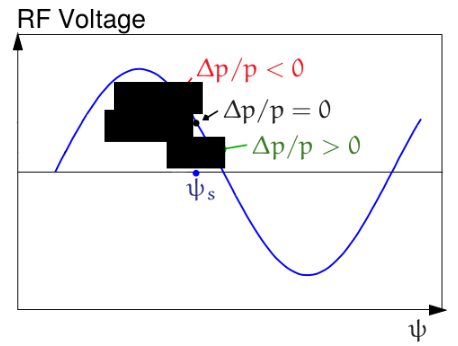
\includegraphics[width=0.4\textwidth]{Figures/RFphase.png}
\caption[Phase focusing]{RF voltage as a function of the RF phase. In the ideal case, the particles arrive at the RF phase $\psi_s$. 
Particles with a smaller momentum ($\Delta$p/p $<$ 0) will arrive later than the ideal particles, and will therefore be accelerated more, particles with larger momentum will be accelerated less respectively.}
\label{fig:RFPhase}
\end{figure}
%To still guarantee the particle to be accelerated by the same RF phase, the RF frequency is varied over the length of the linear collider.

Rolf Wider\o e did not only build the first linear accelerator, he even more importantly invented the very first accelerating structures using electromagnetic fields.
In a magnetic field, the charged particles are deflected on a radial path, which therefore allows the accelerator to be much smaller than before.~\cite[cf. p. 8]{Wilson}
Exactly that idea was needed to advance from purely linear to circular in particle accelerators.

\section{Transversal beam dynamics}
\label{AccPhysics:Magnets}

Circular acceleration does also have certain challenges.
From the equilibrium of the Lorentz and the centripetal force follows:
\begin{align}
q(\vec{v}\times \vec{B}) &= \frac{m\vec{v}^2}{r}\\
qvB\vec{e_r} &= \frac{mv^2}{r}\vec{e_r} \nonumber \\
 r&=\frac{mv}{qB}\\
 &=\frac{p}{qB}\label{eq:MagField_Radius}
\end{align}
Since the momentum $p$ of the charged particle rises over time, the radius $r$ of its circular path increases if the magnetic field $B$ is constant.
The accelerator hence has to be built accordingly taking the increase in the radius into account, or needs to use magnets with variable field strengths.
Latter is done in synchrotron machines, a type of circular accelerator combining the principles of all particle accelerators mentioned above: acceleration in RF cavities, variation of the RF frequency, and variable magnetic field strengths.
In this way, the particles are traveling along a stationary orbit, passing through the same magnets and cavities over and over again until the desired beam energy is reached.
To insure the stability of the orbit, not only bending dipole magnets can be found but also quadrupole magnets for focusing the particles, and sextupole and octupole magnets which then correct orbit fluctuations.
The need for higher order correction magnets can be derived from the expansion of the magnetic field around the ideal path of the particle (x = 0):
\begin{alignat}{5}
 B_y(x) &= B_{y0} &&+ \frac{\partial B_y}{\partial x}x &&+ \frac{1}{2!}\frac{\partial^2 B_y}{\partial x^2}x^2 &&+ \frac{1}{3!}\frac{\partial^3 B_y}{\partial x^3}x^3 &+ ...\\
 \intertext{When multiplying with $\frac{q}{p}$:}
 \frac{q}{p}B_y(x) &= \frac{q}{p}B_{y0} &&+ \frac{q}{p}\frac{\partial B_y}{\partial x}x &&+  \frac{1}{2!}\frac{q}{p}\frac{\partial^2 B_y}{\partial x^2}x^2 &&+ \frac{1}{3!}\frac{q}{p}\frac{\partial^3 B_y}{\partial x^3}x^3 &+ ...\\
  &= \frac{1}{r} &&+ kx &&+ \frac{1}{2!}mx^2 &&+ \frac{1}{3!}ox^3 &+ ... \label{eq:field_components}\\
  &\rightarrow \textnormal{dipole} &&+ \textnormal{quadrupole} &&+ \textnormal{sextupole} &&+ \textnormal{octupole} &+ ...\nonumber
\end{alignat}
Equation~\ref{eq:field_components} shows directly the connection between the radius and the magnetic field in the dipole component (compare with Equation~\ref{eq:MagField_Radius}).
In the quadrupole, sextupole and octupole components, a factor for the magnet strength is introduced.
According to the Maxwell equation $\vec{\nabla}\cdot\vec{B} = \frac{\partial B_y}{\partial x} -\frac{\partial B_x}{\partial y} = 0$, the Lorentz force on a particle in a quadrupole magnet, has therefore to be written as (cf. \cite[p. 372]{VacuumElectronics}):
\begin{multicols}{2}
\noindent 
\begin{align}
 F_x &= -qv\frac{\partial B_x}{\partial y}x \nonumber\\
  &= -q\beta c\frac{\partial B_x}{\partial y}x\\
  &= -gx\label{eq:Quad_Lorentz_x}
\end{align}
\columnbreak
\begin{align}
 F_y &= qv\frac{\partial B_y}{\partial x}y\nonumber \\
  &= q\beta c\frac{\partial B_y}{\partial x}y\\
  &= gy \label{eq:Quad_Lorentz_y}
\end{align}
\end{multicols}
From Equations~\ref{eq:Quad_Lorentz_x} and \ref{eq:Quad_Lorentz_y}, it becomes clear that quadrupoles can only focus in one direction, whilst it defocuses in the other.
A schematic cross-section of a quadrupole magnet is shown in Figure~\ref{fig:Quadrupole}, in which a positively charged particle would be focused in the y-direction and defocused in the x-direction.
The magnetic field lines point from the magnetic north pole to the south pole, and get denser towards the edges of the beam pipe.
The further a beam particle is away from the center, the stronger is the magnetic field it experiences, and the more it is deflected towards the center.
\begin{figure}
\centering
\includegraphics[width=0.4\textwidth]{Figures/Quadrupole.png}
\caption[Cross-section of a quadrupole magnet]{Schematic cross-section of a quadrupole magnet with the four magnetic north and south poles.
The beam pipe is centered in the middle between the pole shoes.
A positively charged particle inside the beam pipe would be focused in the y-direction and defocused in x.~\cite[p. 88]{Hinterberger}}
\label{fig:Quadrupole}
\end{figure}
\\Due to the fact that there are focusing and defocusing quadrupoles, so-called FODO structures are commonly used in particle colliders.
FODO is an alternating structure made out of focusing quadrupole magnets (``F'') and defocusing ones (``D''), with drift paths in between (see Figure~\ref{fig:FODO}).
After several of these structures, which act like optical lenses, the particle beam is focused in both directions, horizontally and vertically.
\begin{figure}
\centering
\includegraphics[width=0.5\textwidth]{Figures/FODO.png}
\caption[Schematic of FODO structure]{Schematic of a FODO structure in the horizontal and vertical plane. The particles are focused and defocused by the quadrupoles that act as lenses. The overall beam envelope is compressed after a certain number of focusing and defocussing quadrupoles.~\cite[p. 65]{Hinterberger}}
\label{fig:FODO}
\end{figure}
Due to the restoring force, particles that were deflected by the focusing magnets start to perform betatron oscillations around the ideal particle path.
The amplitude of these oscillations is the beam envelope that covers the paths of all beam particles, i.e. the maximum transverse beam dimension at a given location.
It can be expressed by the two beam parameters $\beta$ and $\epsilon$ which will be explained in the following:\\
The beta function $\beta$ describes the spatial dependency of the amplitude and the wave length of the betatron oscillations.
It is a periodic function, dependent on the focusing strengths and the order of the magnets in the beam line.
At any given point along the beam line, the $\beta$ value can be given in its units of length.
Of particular interest is its value at the interaction point (IP), the point of the beam collisions, where it is then  named $\beta^*$ .
The smaller the beta function is, the narrower is the beam.\\
Like the beta function, the transverse emittance $\epsilon$ is defined in the horizontal and vertical plane.
$\epsilon$ is a direct measure of the convergence of the beam with respect to its spread in space and in momentum.
A small emittance therefore means that the beam particles are confined to a small space, whilst they are all of the same momentum.
It also has the units of length, and is often given as the normalized emittance $\epsilon^* = \epsilon\gamma$, with the relativistic Lorentz factor $\gamma=\frac{1}{\sqrt{1-v^2/c^2}}$.\\
Together, the spatial amplitude of the betatron oscillations can be written as $\sqrt{\epsilon\beta}$.
Since the amplitude of these oscillations counts towards the size of the beam, it can then be written as $\sigma_{betatron} = \sqrt{\epsilon\beta}$.
The amplitude is also shown as the maximum extent in x in the so-called phase space ellipse, shown in Figure~\ref{fig:PhaseSpaceEllipse}.
The phase space consists of x and x', meaning the position and the momentum of the particles.
The ellipse drawn in the phase space is the region in which the motion of the particles is stable, it illustrates the qualities of the particle beam.
Since the particle's spread in position and momentum varies along the beam line, the shape of the ellipse changes constantly, but the area of the ellipse stays the same.
The variables $\alpha$ and $\gamma$ are defined here as: $\alpha = -\frac12\beta'$ and $\gamma = \frac{1+\alpha^2}{\beta}$.~\cite[cf. p. 283ff]{Wangler}
\begin{figure}[h]
\centering
\includegraphics[width=0.5\textwidth]{Figures/PhaseSpaceEllipse_w_AxisTitles.png}
\caption[Phase space ellipse]{Phase space ellipse~\cite[based on p. 158]{Wiedemann}}
\label{fig:PhaseSpaceEllipse}
\end{figure}
\\The actual transverse size of the beam is not yet fully defined by the spatial amplitude of the betatron oscillations.~\cite[cf. p. 108ff]{Conte}
Also the deviation from the ideal particle trajectory due to the momentum spread has to be taken into account, which is defined by the dispersion function $\eta$.
Like $\epsilon$ and $\beta$, it is dependent on the position along the beam line, and can be defined as $\eta = \frac{dx}{d\delta}$, with the fractional deviation from the ideal particle momentum $x'_0$: $\delta = \Delta x'/x'_0$.
With this knowledge, the overall beam size can now be calculated:
\begin{align}
 \sigma&=\sqrt{\sigma^2_{betatron}+\sigma^2_{dispersion}}\\
 &=\sqrt{\epsilon\cdot\beta+\left(\eta\frac{\Delta x'}{x'_0}\right)^2}
\end{align}

\section{Linear colliders in comparison to circular colliders}
\label{AccPhysics:Linear-Circular}
These transversal beam dynamics, described in the section above, are of course valid for circular as well as linear accelerators.
In both machines, the acceleration with RF cavities, for instance, is accompanied by beam deflections and corrections with the help of magnets.
Naturally, the beam line of a circular collider contains on average more bending magnets than a linear collider.\\
Currently, the world's largest circular particle collider is the Large Hadron Collider (LHC) at CERN in Switzerland, a synchrotron machine with a circumference of \SI{27}{\kilo\meter}.
The collision energy of the two colliding proton beams is \SI{13}{\TeV} in the current run, and its nominal peak luminosity \lumi is \SI{e34}{\centi\meter^{-2}\second^{-1}}.~\cite[p. 3]{LHC_Paper}\\
The collision energy $\sqrt{s}$, or often called center-of-mass energy $E_{cm}$, between the beams with 4-vectors $p_1$ and $p_2$ is calculated as:
\begin{align*}
 s &= (p_1+p_2)^2\\
 &=p_1^2+1p_1p_2+p_2^2\\
 &=m_1^2+2(E_1E_2-\vec{p_1}\vec{p_2})+m_2^2\\
\intertext{In a particle collider, where the beam particles have the same mass $m$ and beam energy $E$:}
&\approx2m^2+2E^2+2|\vec{p}|^2\\
&=4E^2
\end{align*}
The collision energy in a particle collider is therefore $\sqrt{s}=2E$.\\
The luminosity of a particle collider is proportional to the amount of collisions that can occur, and it is defined as:
\begin{align}
 \mathcal{L}&=\frac{N_1N_2 \cdot n_b \cdot f}{2\pi \cdot \sqrt{\sigma^2_{x,1}+\sigma^2_{x,2}} \sqrt{\sigma^2_{y,1}+\sigma^2_{y,2}}}\\
 \intertext{If the bunch sizes of the opposite beams are the same:}
 &=\frac{N_1N_2 \cdot n_b \cdot f}{4\pi \cdot \sigma_x \sigma_y}
\end{align}
$N_{1,2}$ is the number of particles per bunch, which is usually the same for both beams, so that $N_1=N_2$.
$f$ is the revolution frequency, the number of revolutions a bunch makes per second.
$n_{b}$ is the number of bunches, and $\sigma_{x,y}$ is the beam bunch size in the horizontal and the vertical plane.
Table~\ref{tab:ILC_parameters} in Chapter~\ref{ILC} lists these parameters and their values for the LHC in comparison to the International Linear Collider (ILC).
In order to translate the luminosity into an event rate, the luminosity value has to be divided by the cross-section $\sigma_p$ of the physics process that is of interest.
Since the LHC detectors do only measure events from inelastic scattering, the LHC event rate can be calculated by taking only the cross-section for inelastic proton-proton scattering into account, which is measured to be \SI{78}{\milli\barn}~\cite{inelXSection}. Barn (``b'') is the unit of cross-sections in particle physics, and is equivalent to \SI{e-28}{\meter\squared}.
\begin{align}
 \dot{N}&=\mathcal{L}\cdot\sigma_{inelastic}\\
 &=10^{34} \textrm{cm}^{-2}s^{-1} \cdot 78\textrm{\,mb}\\
 &=7.8\times 10^8 s^{-1}
\end{align}
%https://www.lhc-closer.es/taking_a_closer_look_at_lhc/0.cross_section
Per second about 780 million events are occurring at the LHC, because of which it is a so-called ``discovery machine''.
With its high luminosity and high collision energy, the possible physics processes from the hadron collisions cover wide energy ranges.  
New particles, first seen for example as resonance peaks in the measured mass spectra, can be discovered easier due to the large phase space.
This was the case in 2012 for instance, when the LHC found a peak at an energy of \SI{126}{\GeV}, shortly after recognized as the very first measurement of a Higgs boson.~\cite{Higgs}\\
%The reason why large synchrotron rings need pre-accelerators is that the range for changing the magnet's field strength is limited.
Why these so-called ``discovery machines'' are hadron and not lepton colliders, and why they are circular and not linear, is to be explained with the physical qualities of the colliding particles.
Hadrons are by definition composite particles, the actual colliding particles in a collision are therefore their partons, the constituents of the hadrons.
Which energy the single partons have, follows a certain probability function, leading to the fact that the collision energy in hadron colliders can cover a large range.
This so-called deep inelastic scattering is explained in more detail in Chapter~\ref{StandardModel}.\\
In contrast to that, a collision of leptons as elementary particles is the interaction of exactly these leptons at exactly their given energy.
This is one of the reasons why lepton colliders are called ``precision machines''.
Being able to set the collision energy precisely means that the events occurring in lepton colliders can be preselected.\\
The decision whether to build a lepton or a hadron collider therefore depends mainly on the physics goal.
The next question to be answered is which design the collider should have, linear or circular.
Again, both alternatives have clear advantages and disadvantages.
One advantage of circular accelerators was already mentioned before, namely the possibility to go to high energies by simply letting the beams perform more revolutions and hence gain more and more energy from every turn.
This is not possible in linear colliders, since the beams are not used after collision but dumped.
The full collision energy has to be gained in a single go.
The only way to increase the collision energy of a linear collider is to make the accelerating line longer. So, why do linear colliders exist at all?\\
The answer lies in the synchrotron radiation, radiation in the form of photons being emitted by deflecting charged particles.
Every deflection in a magnetic field yields an energy loss in form of this synchrotron light, and the more magnets an accelerator has, the more energy loss the beam suffers from.
The synchrotron radiation power is defined as~\cite[p. 33]{Wille}:
\begin{equation}
 P_S = \frac{e^2c}{6\pi\epsilon_0}\frac{1}{(m_0c^2)^4}\frac{E^4}{R^2}
\end{equation}
This directly leads to the energy loss per turn in a circular collider of radius R, for which one turn takes the time interval $T$:
\begin{align}
 \Delta E &= P_S\cdot T\\
 &= P_S\frac{2\pi R}{c}\\
 &=\frac{e^2}{3\epsilon_0(m_0c^2)^4}\frac{E^4}{R} \label{eq:Eloss_synchrotron_radiation}
\end{align}
In order to counteract the loss, the beam has to be accelerated by at least $\Delta E$ for every turn.
Equation~\ref{eq:Eloss_synchrotron_radiation} also implies that a circular accelerator with high beam energies either has to have accelerating cavities with extremely high gradients, or that its radius has be so large that it can compensate the factor $E^4$.
Having a closer look at the equation, it now becomes clear why the LHC for example is a hadron collider:
Due to the factor $m_0^{-4}$, the synchrotron radiation is much lower for particles with higher masses.
When comparing the LHC (with a radius of \SI{2804}{\meter}) one time with \SI{6.5}{\GeV} beams of protons and another time with electrons, then it can be calculated directly that an ``Electron-LHC'' would lose about 1.14\,$\cdot\,10^{13}$ times as much energy from synchrotron radiation than the existing LHC, simply because of the electron-proton mass ratio:
\begin{align*}
 \frac{\Delta E_e}{\Delta E_p} &= \frac{7.49\cdot10^{10} \textnormal{MeV}}{6.59\cdot10^{-3} \textnormal{MeV}}\\
 &=1.14\cdot10^{13}\\
 &=\frac{m_e^4}{m_p^4}
\end{align*}
Concluding, a circular hadron collider lends itself to be a particle accelerator in the high-energy frontier, whereas a linear lepton collider is destined to be a collider in the precision frontier.

\paragraph{A question of money}
Also the cost for the accelerator might be a deciding factor when considering the design for a future collider.
For the overall expected cost, there is a rough rule of thumb formulated by Burton Richter in 1980. \todo{Find reference to cost argument by B. Richter}
Based on cost estimates of previous accelerators, the cost of circular accelerators tends to grow quadratically with the center-of-mass energy that is aimed for, whilst it grows linearly with the energy for linear colliders.
Strictly speaking, the proportional cost growth for linear colliders is true considering only the accelerating structures, since the achievable energy is increasing linearly with the length of the accelerator.
But there is more to a linear collider than just the accelerating structure: damping rings, focusing systems and beam dumps are only a few examples of what a linear collider layout contains as well.
These elements, which add inevitable basic costs, are explained in more detail in Chapter~\ref{ILC:layout}.\\
Apart from the basic costs, the increase in costs when reaching to higher center-of-mass energies is larger for circular than for linear colliders.
\chapter{Physics of lepton colliders}
\label{Lepton_Physics}
\begin{chapterabstract}
The physics done at particle colliders, where two particle beams are brought into collision, is the physics of atoms and quanta, of nuclei and partons, of particles that build up everything we know, but also of new particles, physics beyond our current knowledge.
After a brief introduction of the Standard Model, a theory describing the elementary particles and the fundamental forces, the physics processes at a lepton collider will be explained in more detail.
\end{chapterabstract}
\newline

Particle physics reaches back to the ancient Greek times, when the idea was developed that matter is made of ``indivisible'' (\'atomos, Greek) parts.
Atoms are, in fact, not indivisible at all.
When the electron was experimentally discovered in 1897 by J.J. Thomson, it was proposed that these particles must be a component of every atom.~\cite[p. 13ff]{Griffiths}
That sparked the interest of many physicists in the early \nth{20} century to perform experiments probing atoms.
One of them was Ernest Rutherford, who fired alpha particles\footnote{An alpha particle is the nuclei of a Helium atom. Ernest Rutherford obtained them from radioactive decays of uranium amongst others.} through a thin gold foil, and thereby found that atoms are mostly empty with a positively charged nucleus that is only a fraction of the size of the atom itself.
This discovery was a crucial step towards the modern atomic model.\\
Close to our current understanding of the atomic model is the Bohr model, developed by Niels Bohr in 1914.~\cite[p. 15]{Griffiths}
It describes that electrons orbit the positively charged nucleus on stable shells with distinct radii.
The shells correspond to discrete energies, such that an electron switching from one shell to a shell with a larger radius would have to absorb energy, or emit energy respectively.
This energy quantum is absorbed or emitted in form of light, more precisely in form of a photon.
Nowadays, it is known that the electrons do not orbit the nucleus on discrete shells but rather in orbital zones, where the electron has a higher probability to be observed.\\
In order for an atom to have a neutral charge, the number of electrons in the atomic shells have to be balanced by an equal amount of positive charge of the nucleus.
That nuclei of different atoms are built from the hydrogen nucleus was already proven by Rutherford.
He thereby discovered the proton, and explained that the positive charge of the nucleus is the summed up charges of the protons inside the nucleus.\\
In 1932, it was found that atoms can not only consist of electrons and protons.~\cite[p. 15]{Griffiths}
The mass measurements of various isotopes showed that their masses differ by concrete amounts.
The explanation was that the nucleus must consists of protons and particles with a similar mass but a neutral charge, the neutrons.
Isotopes are therefore atoms of the same element with the same number of protons, but with a different amount of neutrons.\\
Over the years, the development of particle accelerators that can accelerate particles to higher and higher energies allowed to probe even the constituents of the atom.
This showed that the end has not been reached yet, that protons and neutrons are not elementary but composite particles.
Their partons, the so-called quarks, are part of the current theory of all elementary particles and the fundamental forces they interact with, the Standard Model.
\section{The Standard Model}
\label{StandardModel}
The Standard Model (SM) was developed and formulated around the 1960s and 1970s, when the theories of quantum electrodynamics (QED) and of quantum chromodynamics (QCD) were combined into one mathematical model that explains how the elementary particles interact with each other via the fundamental forces of the universe.~\cite[p. 3]{Griffiths}
Since then, high-energy particle physics experiments could verify the SM predictions so that it has proven itself to be currently the best theoretical model of all subatomic particles we know of.\\
The SM differs between two classes of the fundamental particles: 
the particles that make up all matter are called \textit{fermions}, whilst the force mediators, through which the fermions can interact, are called \textit{gauge bosons}.
\begin{figure}[h]
\centering
\includegraphics[width=0.6\textwidth]{Figures/Standard_Model_of_Elementary_Particles.png}
\caption[Standard Model]{The Standard Model describes all elementary particles, the twelve fermions in their three generations and the four gauge bosons, as well as the Higgs boson.
The shadows indicate possible interactions between the fermions and gauge bosons.~\cite{SM}}
\label{fig:SM}
\end{figure}

\paragraph{Fermions}
Fermions are particles with a spin quantum number of $s = 1/2$. 
The spin is the particle's rotation about its central axis, and has a direction and a specific amplitude.
The amplitude can be calculated as $\frac{h}{2\pi}\sqrt{s(s+1)}$, with $h$ being the Planck constant.~\cite[p. 121]{Griffiths}
All fermions have a specific set of quantum numbers, so that by giving the electric charge, the spin, and the flavor,  all fermions can be identified precisely.
Table~\ref{tab:Fermions} lists all Standard Model fermions with their quantum numbers.

\begin{table}
\caption[Quantum numbers of the Standard Model fermions]{Quantum numbers of the Standard Model fermions. The table lists the values for the electric charge $q$, and the spin $s$ for all fermions, as well as the lepton number $L$ of the leptons and the quark flavor of the quarks. Their respective antiparticles are highlighted by the shaded background.~\cite[cf. p. 49]{Griffiths}}
\label{tab:Fermions}
\centering
\begin{tabularx}{\textwidth}{c|c|rrrrr|@{\hskip 0.03in}|c|rrrrrrrr}
\hline\hline
& Leptons & $q$ & $s$ & $L_e$ & $L_{\mu}$ & $L_{\tau}$ & Quarks & $q$ & $s$ & $U$ & $D$ & $C$ & $S$ & $T$ & $B$\\
\hline
& e\textsuperscript{--} & --1 & 1/2 & +1 & 0 & 0 & u & +2/3 & 1/2 & +1 & 0 & 0 & 0 & 0 & 0\\
\rowcolor{Gray}
\cellcolor{white}& e\textsuperscript{+} & +1 & 1/2 & --1 & 0 & 0 & $\bar{\rm{u}}$ & --2/3 & 1/2 & --1 & 0 & 0 & 0 & 0 & 0\\
& $\upnu$\textsubscript{e} & 0 & 1/2 & +1 & 0 & 0 & d & --1/3 & 1/2 & 0 & --1 & 0 & 0 & 0 & 0\\
\rowcolor{Gray}
\multirow{-4}{*}{\rotatebox[origin=c]{90}{\parbox[c]{1.9cm}{\cellcolor{white}\centering First generation}}} &$\bar\upnu$\textsubscript{e} & 0 & 1/2 & --1 & 0 & 0 & $\bar{\rm{d}}$ & +1/3 & 1/2 & 0 & +1 & 0 & 0 & 0 & 0\\
\hline
& $\upmu$\textsuperscript{--} & --1 & 1/2 & 0 & +1 & 0 & c & +2/3 & 1/2 & 0 & 0 & +1 & 0 & 0 & 0\\
\rowcolor{Gray}
\cellcolor{white}&$\upmu$\textsuperscript{+} & +1 & 1/2 & 0 & --1 & 0 & $\bar{\rm{c}}$ & --2/3 & 1/2 & 0 & 0 & --1 & 0 & 0 & 0\\
& $\upnu$\textsubscript{$\upmu$} & 0 & 1/2 & 0 & +1 & 0 & s & --1/3 & 1/2 & 0 & 0 & 0 & --1 & 0 & 0\\
\rowcolor{Gray}
\multirow{-4}{*}{\rotatebox[origin=c]{90}{\parbox[c]{1.9cm}{\cellcolor{white}\centering Second generation}}}& $\bar\upnu$\textsubscript{$\upmu$} & 0 & 1/2 & 0 & --1 & 0  & $\bar{\rm{s}}$ & +1/3 & 1/2 & 0 & 0 & 0 & +1 & 0 & 0\\
\hline
& $\uptau$\textsuperscript{--} & --1 & 1/2 & 0 & 0 & +1 & t & +2/3 & 1/2 & 0 & 0 & 0 & 0 & +1 & 0\\
\rowcolor{Gray}
\cellcolor{white}& $\uptau$\textsuperscript{+} & +1 & 1/2 & 0 & 0 & --1 & $\bar{\rm{t}}$ & --2/3 & 1/2 & 0 & 0 & 0 & 0 & --1 & 0\\
& $\upnu$\textsubscript{$\uptau$} & 0 & 1/2 & 0 & 0 & +1 & b & --1/3 & 1/2 & 0 & 0 & 0 & 0 & 0 & --1\\
\rowcolor{Gray}
\multirow{-4}{*}{\rotatebox[origin=c]{90}{\parbox[c]{1.9cm}{\cellcolor{white}\centering Third generation}}}& $\bar\upnu$\textsubscript{$\uptau$} & 0 & 1/2 & 0 & 0 & --1 & $\bar{\rm{b}}$ & +1/3 & 1/2 & 0 & 0 & 0 & 0 & 0 & +1\\
\hline\hline
\end{tabularx}
\end{table}

Fermions are further categorized as \textit{leptons} and \textit{quarks}, as well as in three generations, which can be seen in Figure~\ref{fig:SM}.
Among the leptons, there are the electron and its heavier brothers, the muon and the tau.
In their respective generation, each of them has a neutrino, hence there are the electron-neutrino, muon-neutrino, and tau-neutrino, which are electrically neutral particles.\\
Since the SM does in general not remark the corresponding antiparticles, there are actually not only six leptons but twelve.
The only difference between particles and antiparticles is the sign of their internal quantum numbers:
The electron's antiparticle is the positron, which has the same mass and spin as the electron, but has a positive charge of +1, and a negative lepton number $L_e$ of -1.
The antiparticles of the muon ($\upmu$\textsuperscript{-}) and the tau ($\uptau$\textsuperscript{-}) hence are $\upmu$\textsuperscript{+} and $\uptau$\textsuperscript{+}, respectively.
As neutrinos on the other hand have no electric charge, they can only be distinguished from their respective antineutrino by their lepton number and their helicity.
The helicity describes the state of the particle's spin direction in comparison to the particle's momentum.
When the spin direction and the momentum are parallel, the particle is called right-handed.
It is called left-handed, when they are antiparallel.
In the SM, neutrinos are always left-handed, whilst antineutrinos are right-handed.
So far, no experiment has shown the opposite.\\
Every generation of quarks consists of one up- and one down-type quark, where the up-type quarks have an electric charge of 2/3, whilst down-type quarks have a charge of --1/3.
However, they do not only carry the electric charge, but also the so-called color charge.
Every quark has one of three colors (red, green, and blue), every antiquark has one of three anti-colors (anti-red, anti-green, and anti-blue).
Thus, there are overall 36 different quarks and antiquarks.
Due to the physics law of confinement, there can only be color-neutral particles.
Quarks are therefore not free, but hadronize and form a bound state together with other quarks.
These bound quark states, called hadrons, consist of either two, three, or five quarks.
A particle with a quark of a specific color and an antiquark of the corresponding anti-color is called a meson.
A baryon, which is a particle with three quarks, can only be color-neutral when it carries three quarks with three different colors (or anti-colors), so red--green--blue or anti-red--anti-green-anti--blue.
Any other combination is not possible.
Finally, the penta-quarks are bound states from five quarks, where three of them form a color triplet like a baryon, and the remaining two form a color-anticolor pair like a meson.\\
In everyday nature, the only observable hadrons are the protons and neutrons.
They are baryons, hence are built from three quarks:
protons contain two up-quarks and one down-quark, giving the proton its positive electric charge of +1.
Neutrons on the other hand are formed by one up-quark and two down-quarks, resulting in an electrically neutral particle. 
Together, they construct the nuclei of every atom of every element.
%The masses of the quarks increases towards higher generations.

\paragraph{Bosons}
Other than fermions, gauge bosons are particles with a spin of +1.
The gauge bosons described in the SM are the force mediators of the fundamental forces of nature, except gravity.
The fermions explained above are subject to the fundamental forces, and can interact with each other by exchanging these gauge bosons.\\
The photon is a massless particle mediating the electromagnetic force.
Gluons are massless particles as well.
They carry the strong force, and are like the quarks also color-charged.
Therefore they cannot occur in isolation.
W and Z bosons on the other hand are massive particles, which are responsible for the weak force.\\
Gravity is the only fundamental force that is not represented by the SM.
On the scale of particle physics, it is by far the weakest force.

In contrast to the gauge bosons, the Higgs boson has not got a spin of +1, but a sping of 0.
It is therefore a scalar boson.
The Higgs is the mediator of the Higgs field which is responsible for giving the mass to massive particles.

\section{Production modes}
\label{Production_modes}

\begin{figure}
\centering
\begin{subfigure}[b]{0.4\textwidth}
\includegraphics[width=\textwidth]{Figures/ILC_cross_section.png}
\caption{\positron \electron cross-section~\cite{ILC_cross}}
\end{subfigure}
\begin{subfigure}[b]{0.4\textwidth}
\includegraphics[width=\textwidth]{Figures/LHC_cross_section.pdf}
\caption{pp cross-section~\cite{LHC_cross}}
\end{subfigure}
\caption[Cross-sections for ILC and LHC]{Cross-section at \positron \electron and pp colliders as a function of the collision energy.}
\label{fig:Cross_sections}
\end{figure}

\section{Backgrounds}
\label{Backgrounds}
\subsection{High cross-section backgrounds from beam-beam interactions}
\label{BeamBeam}
\subsubsection{Pair background}
\label{BeamBeam:pairs}
\todo{Re-write this paragraph}
%Found here: http://www.sciencedirect.com/science/article/pii/S0168900216310919
For a Gaussian beam, the average energy $E_{\gamma}$ of photons from the deflection of the colliding particles is proportional to [5]:
\begin{equation}
 E_{\gamma} \propto \frac{N}{(\sigma_x+\sigma_y)\sigma_z}
 \label{eq:pair_energy}
\end{equation}
where N is the number of particles per bunch. The average number of photons is proportional to:
\begin{equation}
 n_{\gamma} \propto \frac{N}{(\sigma_x+\sigma_y)}
 \label{eq:pair_number}
\end{equation}
%Therefore, in ILC chapter about beam parameters: Hence flat beams with $\sigma_x\gg\sigma_y$ are used. The product of the horizontal and vertical beam sizes is small leading to high luminosity while the sum of them is large, reducing the beamstrahlung effect.

\begin{figure}
\begin{subfigure}[b]{0.33\textwidth}
\includegraphics[width=\textwidth]{Figures/Bethe-Heitler.pdf}
\caption{Bethe-Heitler}
\end{subfigure}
\begin{subfigure}[b]{0.33\textwidth}
\includegraphics[width=\textwidth]{Figures/Breit-Wheeler.pdf}
\caption{Breit-Wheeler}
\end{subfigure}
\begin{subfigure}[b]{0.33\textwidth}
\includegraphics[width=\textwidth]{Figures/Landau-Lifshitz.pdf}
\caption{Landau-Lifschitz}
\end{subfigure}
\caption[LO Feynman diagrams of the production of the background pairs.]{The LO Feynman diagrams of the production processes of the background pairs: Bethe-Heitler, Breit-Wheeler and Landau-Lifschitz.}
\label{fig:Feynman:pair_production}
\end{figure}

\subsubsection{Bhabha scattering and $\gamma\gamma\rightarrow$hadrons}
\label{BeamBeam:bhabha_gammagamma}

\begin{figure}
\centering
\begin{subfigure}[b]{0.35\textwidth}
\includegraphics[width=\textwidth]{Figures/bhabha_scattering.pdf}
\caption{Bhabha scattering}
\end{subfigure}
\vspace*{0.2cm}
\begin{subfigure}[b]{0.35\textwidth}
\includegraphics[width=\textwidth]{Figures/gammagamma_hadrons.pdf}
\caption{$\gamma\gamma\rightarrow$hadrons}
\end{subfigure}
\caption[LO Feynman diagrams of bhabha scattering and the $\gamma\gamma\rightarrow$hadrons process.]{The LO Feynman diagrams of the bhabha scattering and the $\gamma\gamma\rightarrow$hadrons process.}
\label{fig:Feynman:bhabha_gammagamma}
\end{figure}

\subsection{Machine backgrounds}
\label{MachineBackgrounds}
\chapter{The International Linear Collider}
\label{ILC}
The International Linear Collider (ILC) is a linear \electron \positron accelerator with an center-of-mass energy of \unit{500}{GeV} in the first stage and \unit{1}{TeV} in the second.
The state of the art technologies for both, the detectors and the machine, and the machine design make a clean environment and high precision measurements possible, because of which the ILC will be a unique machine.\\
The following sections will talk about the ILC layout, its possible sites, the two detectors, and finally the physics motivation for such a capable accelerator.
\section{Layout}
\label{ILC:layout}

Figure~\ref{fig:ILC_Layout} shows the schmeatic layout of the ILC for the \unit{500}{GeV} stage.
The electrons originate in the polarised source based on a photocathode DC gun.
When these electrons pass through an undulator, high-energy photons are produced which are then converted to electron-positron pairs.
This is the polarised positron source.
The main linacs are extendable for the machine upgrade to \unit{1}{TeV}.

\begin{figure}
\centering
\includegraphics[width=0.8\textwidth]{Figures/ILC_layout.png}
\caption[Schematic layout of the ILC]{Schematic layout of the ILC~\cite[p. 9]{ILC1}}
\label{fig:ILC_Layout}
\end{figure}


\section{Possible Site}
\label{ILC:site}
\section{SiD and ILD}
\label{ILC:detectors}
\section{Physics Motivation}
\label{ILC:physicsmotivation}

%\chapter{Background simulation tools}


\section{GuineaPig}

\section{Pythia}

\section{MUCARLO}

\section{BDSIM}

\section{FLUKA}
\chapter{BDS and Final-Focus system as background sources}
\section{Background from a Beam Halo Collimator in Final-Focus system}
\subsection{Beam Halo Collimator}
Picture: Collimator drawing\\
Picture: Pictures of installed collimator
\subsection{ATF2}
Picture: ATF2 schematic
\subsection{BDSIM}
%---------------------------------------------------
\subsection{Background studies}
\subsubsection{RHUL Cherenkov detector}
Pictures: setup\\
\begin{figure}
\centering
\includegraphics[width=\textwidth]{AverageNoise_perVoltage.pdf}
\caption[RHUL Cherenkov detector noise]{Average noise signal as a function of the voltage applied to the detector PMT. The noise was measured when the ATF beam was turned off. For each voltage, 500 or 1000 ADC pulses of noise were recorded, and the noise averaged over the number of pulses. The error bars to the mean values are the standard deviation of the mean.}
\label{fig:AverageNoise}
\end{figure}
Figure ~\ref{fig:AverageNoise} shows the mean values of the noise measurements for different PMT voltages. For every point either 500 or 1000 ADC pulses were recorded and averaged. The error bars represent the standard deviation on the mean value calculated by $SD=\frac{\sigma}{\sqrt{N}}$, where $\sigma$ is the RMS of the noise distribution at each point and N the number of pulses.\\
At around \SI{800}{\volt} the effect of dark current in the PMT starts getting prominent wherefore the noise rises exponentially. For the data shown in the following, the noise is already subtracted. As the data was taken only for these voltages, for which noise measurements were done, the mean value of noise is subtracted from every signal pulse appropriately. Therefore the rise in noise is automatically taken into account for higher voltages.

\subsubsection{Collimator apertures scan - for different intensities and vacuum pressures}
The two jaws of the vertical beam halo collimator can be moved individually. Scans of the background for different collimator apertures were done, first for symmetric positions of the lower and upper jaw around the centre, later for asymmetric positions. Additionally, a scan was done with one jaw fully extracted and the other one moving to certain positions. The last scan is referred to as the 'half aperture scan', whereas the first two scans are the 'symmetric' and the 'asymmetric' scans.\\
Figure ~\ref{fig:AverageSignal_Aperture_BeamIntensities} shows the plot of the average detector signals for the asymmetric scan of different collimator apertures. The scans were done for five different beam intensities. It is clear that the background level rises with increase in intensity. The characteristic shape of the scan is however conserved: the background level is constant while closing the collimator from a full aperture of \SI{24}{\milli\metre} to about \SI{12}{\milli\metre}. When closing to \SI{10}{\milli\metre} the background level drops, and rises again when closing the collimator completely, i.e. to \SI{6}{\milli\metre} full aperture. This characteristic drop and rise between 12 and \SI{6}{\milli\metre} is on the one hand proof of the proper functionality of moving the collimator jaws, on the other hand leaves some questions open: where are the background particles originating that are cut away by the collimator, and does the rise in background mean that the collimator is showering the beam halo particles? Which qualities do these produced background particles have?\\
These questions are addressed in Chapter ~\ref{sec:BDSIM_sim}, in which the effect of the collimator is simulated in a BDSIM simulation.
\begin{figure}
\centering
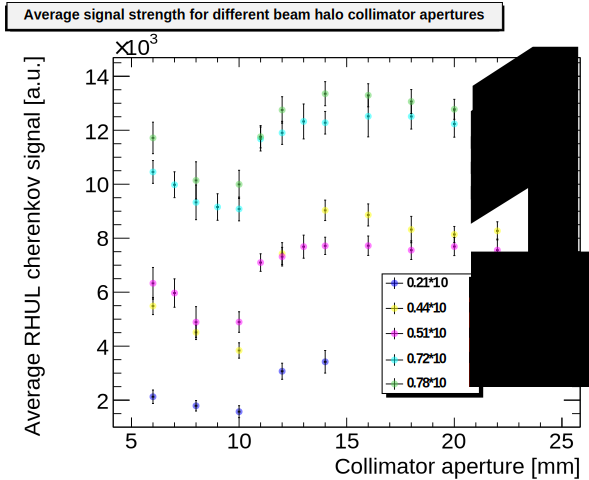
\includegraphics[width=\textwidth]{AverageSignal_perAperture.pdf}
\caption[RHUL Cherenkov detector signal vs. collimator aperture: different beam intensities]{Average signal as a function of the full aperture of the vertical beam halo collimator. The signal was measured for different beam intensities [\num{10e10}]: 0.21, 0.44, 0.51, 0.72 and 0.78, while the PMT voltage was constant at \SI{900}{\volt}. For each aperture, 500 ADC pulses were recorded, and the signal was averaged over the number of pulses. The error bars to the mean values are the standard deviation of the signal distributions at each point.\\For some scans, the data was not taken for all apertures. Therefore, especially the graph for the beam intensity of \num{0.21e10} is missing data points for the half millimetre steps and between 14 and \SI{24}{\milli\metre}.}
\label{fig:AverageSignal_Aperture_BeamIntensities}
\end{figure}
\begin{figure}
\centering
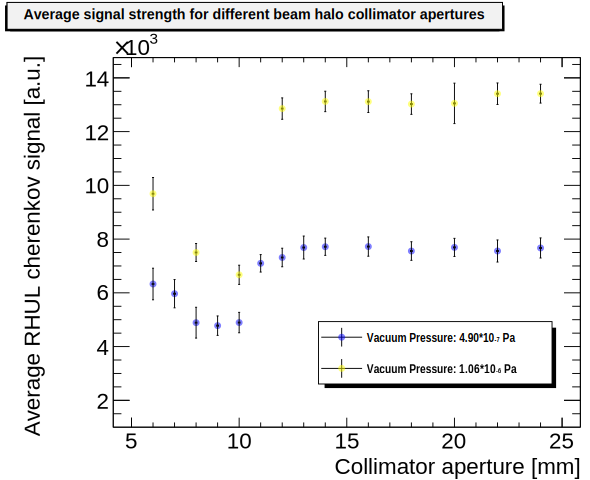
\includegraphics[width=\textwidth]{AverageSignal_perAperture_VacuumPressures.pdf}
\caption[RHUL Cherenkov detector signal vs. collimator aperture: different vacuum pressures]{Average signal as a function of the full aperture of the vertical beam halo collimator. The signal was measured for a beam intensity of \num{0.5e10} and a PMT voltage of \SI{900}{\volt}. The vacuum pressure was lowered from \SI{4.9e-7}{\pascal} to \SI{1.06e-6}{\pascal}. For each aperture, 500 ADC pulses were recorded, and the signal was averaged over the number of pulses. The error bars to the mean values are the standard deviation of the signal distributions at each point.}
\label{fig:AverageSignal_Aperture_VacuumPressures}
\end{figure}
\subsubsection{Test collimator alignment wrt beam position}
\begin{figure}
\centering
\includegraphics[width=\textwidth]{AverageSignal_perJawPosition.pdf}
\caption[RHUL Cherenkov detector signal vs. collimator half aperture]{Average signal as a function of the position of the upper/lower jaw of the vertical beam halo collimator. The signal was measured for a beam intensity of \num{1.05e10} and a PMT voltage of \SI{800}{\volt}. First, the lower jaw was fixed to its open position (\SI{12}{\milli\metre}) and the upper jaw was moved to the positions plotted, then vice versa. For each jaw position, 500 ADC pulses were recorded, and the signal was averaged over the number of pulses. The error bars to the mean values are the standard deviation of the signal distributions at each point.}
\label{fig:AverageSignal_HalfAperture}
\end{figure}
\begin{figure}
\begin{subfigure}[b]{0.5\textwidth}
\includegraphics[width=\textwidth]{AsymmetricScan_4mm_beamintensity084_lego.pdf}
\end{subfigure}
\begin{subfigure}[b]{0.5\textwidth}
\includegraphics[width=\textwidth]{AsymmetricScan_4mm_beamintensity084_colz.pdf}
\end{subfigure}
\caption[RHUL Cherenkov detector signal for certain upper/lower jaw positions]{Average signal as a function of the position of the upper and lower jaw of the vertical beam halo collimator. The signal was measured for a beam intensity of \num{0.84e10} and a PMT voltage of \SI{900}{\volt}. The jaws were moved simultaniously around \SI{4}{\milli\metre}. For each jaw position, at least 500 ADC pulses were recorded, and the signal was averaged over the number of pulses. The content of the bins were set to the appropriat average signal strength at that point.}
\label{fig:AverageSignal_Asymmetric}
\end{figure}
%---------------------------------------------------
\subsection{Collimator as background source}
\label{sec:BDSIM_sim}
\subsection{Effect on background level at IP}

%---------------------------------------------------
\section{Background from a Muon Spoilers}
\subsection{MUCARLO}

\chapter{Background from the main beam dumps}
\label{BeamDumps}

\begin{chapterabstract}
 After every beam collision, the beams of a linear collider are dumped into the main beam dumps.
 For the International Linear Collider, the main beam dump design is based on a water tank, which is tailored to absorb the beam power over a length of about \textit{\SI[detect-all]{12}{\meter}}.
 The first part of this chapter is focused on the irradiation of the water tank and its surrounding, as well as on the neutrons that are produced due to the interaction of the beam particles with the water molecules.
 The second part of this chapter discusses those neutrons which are directed backwards and reach the interaction region.
 They present an additional background for the experiments.
 In the end, suggestions for alternative beam dump designs are given.
\end{chapterabstract}

The spent \positron\electron beams are directed through the extraction line (EXT) of the ILC towards the main beam dumps. 
As can be seen in Figure~\ref{fig:BeamDumps:IP_to_Dump}, the beam dump halls are about \SI{300}{\meter} away from the interaction point (IP) in a direct line of sight.
The extraction lines have the task to transport the highly disrupted beams to the dumps, because of which their quadrupole magnets have a large acceptance for offsets in the beam orbit as well as in the beam momentum of up to \SI{60}{\percent}~\cite[p. 139]{TDR32}.
The quadrupole magnets are to minimize beam loss so that additional diagnostic devices in the EXT lines can measure the qualities of beam bunches before they are dumped.
\begin{figure}
\centering
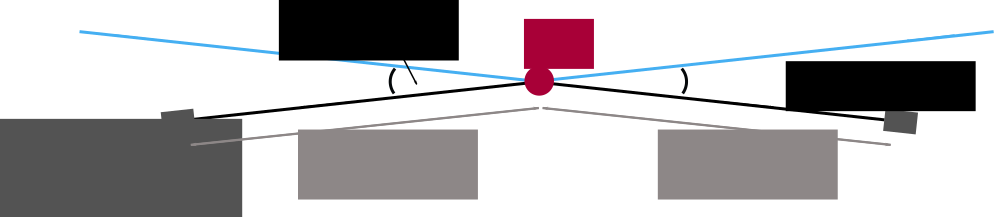
\includegraphics[width=0.6\textwidth]{Figures/BeamDump/IP_EXT.png}
\caption[Schematic of the ILC interaction region with extraction line]{Illustration of the interaction region of the ILC with the extraction line (EXT) leading from the IP to the main beam dump halls.
The extraction lines are about \SI[detect-all]{300}{\meter} long.
The illustration is not to scale.}
\label{fig:BeamDumps:IP_to_Dump}
\end{figure}
The beam dumps basically consist of tanks, filled with water at a pressure of \SI{10}{\bar} and surrounded by iron and concrete shieldings. 
The choice of a water tank as the beam dump is based on the high specific heat capacity of water, which is ideal to dissipate the energy of the beams. 
Therefore the water beam dumps for the ILC are designed to absorb the beam power of \SI{17}{\mega\watt} at \SI{500}{\GeV} centre of mass energy.\\
Dumping a high energy lepton beam in a water tank means on the other hand the emission of neutrons of high and low energies. 
Not only the effect of these neutrons reaching back to the detectors at the interaction point, but also the doses that the surrounding area would suffer from, are the centre of interest in this chapter. 
The higher occupancy in the detectors is a small effect of the neutrons, whereas the damage of the detector components and the irradiation of the surrounding are the more severe consequences. Neutron background would on the one hand lead to displacement damage in the silicon sensors, which results in charge traps, reduction of charge transfer and the overall degrading of the detector performance. 
On the other hand, the irradiation of the surrounding leads to restricted access of the accelerator tunnel and activates all present components.
\\It is therefore crucial to understand the level of neutron background generated by every beam bump of the ILC beam trains.

\section{\fluka and \flair}
\label{BeamDumps:fluka}
\fluka~\cite{FLUKA,FLUKA2} is known to be a very accurate Monte Carlo simulation tool in respect of simulating low energy neutrons. 
After providing the simulation settings and the geometry in a text file as input source, \fluka uses certain algorithms to simulate and track the particles through the geometry.
%TODO: FLUKA algorithms
The graphical interface developed for \fluka is called \flair~\cite{FLAIR}. 
Its plug-in flair-geoviewer allows interactive geometry viewing and editing, as well as debugging and three dimensional visualization.

\section{Beam dump design}
\label{BeamDumps:design}
The design for the beam dump simulated for this thesis is based on the TDR design as well as on the technical design drawings done by B. Smith~\cite{Smith_drawings}.
Figure~\ref{fig:BeamDumps:geometry} shows the visualization of the beam dumps modelled within \fluka. It is a simplified version derived from the design drawings, only containing a simple water tank in the middle of the shielding in the beam dump tomb. The infrastructure, like cables, water pipes etc., is not included in the simulation geometry.

\begin{figure}
\begin{center}
\resizebox{.9\textwidth}{!}{%
\includegraphics[height=0.35\textheight]{Figures/BeamDump/Front_view_BeamDump_Tomb.png}%
\quad
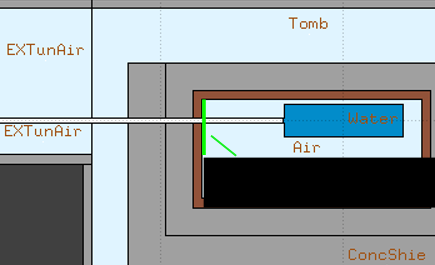
\includegraphics[height=0.35\textheight]{Figures/BeamDump/Bird_view_BeamDump_Tomb.png}%
}
\caption[Geometry of the simulated beam dumps.]{The beam dumps modelled within \fluka and visualized with \flair. On the left hand side, the front view on the beam dump is shown, i.e. the beam direction is going into the paper plane, whereas the right hand side shows the top view. The actual dump is represented by the water tank in the middle of the different shielding walls. A \fluka specific feature is the need of having a black body void around the geometry. This void is the limit of the tracking region and stops all particles reaching this edge.}
\label{fig:BeamDumps:geometry}
\end{center}
\end{figure}

\section{Simulation studies of the beam dump surrounding}
\label{BeamDumps:sim_surrounding}

\begin{itemize}
 \item Energy deposition for both designs - done
 \item Dose rate for both designs - done 
 \item Particle fluxes for both designs - done 
 \item Number for certain subregions - almost done
 \item Neutron spatial distributions - almost done
\end{itemize}


\section{Simulation studies of extraction line}
\label{BeamDumps:sim_EXT}

\begin{itemize}
 \item Extraction line lattice - explain components
 \item Simulation of neutrons through EXT - not done yet
\end{itemize}

\section{SiD Occupancy study from beam dump neutrons}
\label{BeamDumps:SiDocc}

\begin{itemize}
 \item Occupancy study of neutrons in SiD - not done yet
\end{itemize}
\chapter{\positron\electron pair background as the largest background contribution}
\label{PairBkg}

\begin{chapterabstract}
 At the International Linear Collider, the collision of the two lepton beams goes hand in hand with the production of background particles.
 Unlike at hadron colliders, the main background contribution does not arise from QCD processes and underlying events, but rather from the interaction of the colliding beam's electromagnetic fields.
 The created secondary \positron\electron pairs form a significant background, the so-called pair background, for the inner detectors, and therefore need to be studied in great detail.
 This chapter discusses the effect of the ILC beam parameters on the pair background, and the impact of the \positron\electron pairs on the \sid detector.
\end{chapterabstract}

As discussed in Section~\ref{BeamBeam}, the pair background is a high cross section process from beam-beam interactions and the main source of background at the ILC.
The secondary electrons and positrons show a characteristic density distribution, which reach to the inner layers of the \sid vertex and tracking detectors.
The impact on the \sid detector is studied with respect to the timing, the hit distribution, and the arising detector occupancy.
These impacts are, however, affected by the change in the ILC beam parameters for the ILC250 stage, which is another study done for this thesis and is explained throughout the following sections.
The results of these studies contributed towards design choices of the accelerator and the \sid detector.

\section{The background generator GuineaPig}
\label{PairBkg:GuineaPig}
For studying the effects of the pair background, \positron\electron pairs from beam-beam interactions were generated with the Monte Carlo (MC) background event generator \guineapig~\cite{Schulte:1997nga} version 1.4.4. 
When providing the accelerator beam parameters, the pair background events of one bunch crossing are simulated and stored in an ASCII output file named ``pairs.dat''.
The parameters used for generating the pair background for this thesis are given in Appendix~\ref{Appendix:Pairs:GuineaPig}. 
\\Since the ASCII files cannot directly serve as input to a full \geant~\cite{geant_ref,geant_ref2} detector simulation, a conversion tool was written in context of this thesis, and instructions on its usage are available in~\cite{Confluence}. 
The tool converts the ASCII output to one of the following common file formats: stdhep or slcio~\cite{LCIO}.
These file formats are directly applicable with the \geant based simulation tool \slic~\cite{Graf:2006ei}, which simulates interactions of the input particles with matter.
The geometry of the simulated world is described in a lcdd file in a human-readable format.
The flexible geometry description allows the simulation of particle interactions with individual detector geometries.
To this end, the geometry description file ``sidloi3'' of the \sid detector, which was used for the simulation studies in this and in the following chapters, is based on the detector design described in Section~\ref{ILC:SiD} and in~\cite[p. 69 ff]{TDR4}.

\section{Pair background envelopes}
\label{PairBkg:helix}
Analyzing the generated pair background events, it becomes apparent that the \positron\electron pairs have a low transverse momentum.
Figure~\ref{fig:PairBkg:Momentum} shows the distribution of their longitudinal and transverse momentum for the two ILC stages at \SI{250}{\GeV} and \SI{500}{\GeV} center-of-mass energy.
The longitunal momentum of the \positron\electron pairs reaches roughly \SI{80}{\percent} of the beam energy, whilst the transverse momentum extends to only \SI{0.8}{\GeV} for the ILC250, and \SI{1.6}{\GeV} for the ILC500.
 \begin{figure}[h]
 \centering
  \begin{subfigure}[b]{0.49\textwidth}
   \centering
    \includegraphics[width=0.95\textwidth]{Figures/Pairs/250_500_pairs_comparison_Pz.png}
   \caption{Longitudinal momentum}
   \end{subfigure}
   \hfill
    \begin{subfigure}[b]{0.49\textwidth}
   \centering
    \includegraphics[width=0.96\textwidth]{Figures/Pairs/250_500_pairs_comparison_PT.png}
   \caption{Transverse momentum}
   \end{subfigure}
   \caption[Pair background momentum distributions]{Comparison of the pair background momentum distributions for the ILC at \SI{250}{\GeV} and \SI{250}{\GeV} center-of-mass energy, with the longitudinal momentum shown in Figure (a) and the transverse momentum in Figure (b).}
   \label{fig:PairBkg:Momentum}
 \end{figure}
\\Due to their low transverse momentum, the pairs are deflected on helical tracks in the magnetic field of the detector solenoid magnet.
An algorithm was written that calculates the helix tracks of the pair particles using their four-vectors.
The track positions are computed from the radius of the helix, its center position and its pitch. The following assumptions were made for the algorithm:
The magnetic field in the proximity of the IP is homogeneous, with a field strength of \SI{5}{\tesla} for the SiD solenoid.
The particle momenta do not change in the region of interest for this analysis, because of which the helix radius is constant.
Any particle interaction with other particles or with matter is not taken into account.
\\Figure~\ref{fig:helix_circle} shows schematically the projection of a helix onto the xy-plane.
Depending on the particle's charge the orientation of the helix is determined.
\begin{figure}
    \centering
    \includegraphics[width=0.3\textwidth]{Figures/Pairs/Helix_explanation.png}
    \caption[Schematic projection of the helix on the xy-plane]{
    This schematic shows the projection of a helix track onto the xy-plane, with the vector of the transverse momentum (P\textsubscript{T}) and the the x- and y-momenta (p\textsubscript{x} and p\textsubscript{y}).
    Depending on the particle's charge, the direction of the rotation is either clockwise or anticlockwise.
    The center, the radius, and the orientation of the projected circle is dependent on the transverse momentum of the particle.
    }
    \label{fig:helix_circle}
\end{figure}
The pair density is then plotted using the helix track algorithm to calculate the position in x and y for a given position in z.
For the ILC stage at \SI{500}{\GeV}, the pair background was generated with \guineapig, and its density plotted in Figure~\ref{fig:PairBkg:Density} (a).
The density distribution of all the tracks shows a characteristic bell shape, with the highest density along the z axis.
Since the bell shaped envelope is fully symmetrical in positive and negative z-direction as well as in the xz and yz-plane, the chosen view of the pair background envelopes will in the following always be of the xz-plane in positive z-direction.
 \begin{figure}[!h]
 \centering
  \begin{subfigure}[b]{0.49\textwidth}
   \centering
    \includegraphics[width=\textwidth]{Figures/Pairs/Helix_tracks_xz_80bunches_500GeV_5T.png}
   \caption{Pair backgound density for the ILC500}
   \end{subfigure}
   \hfill
    \begin{subfigure}[b]{0.49\textwidth}
   \centering
    \includegraphics[width=\textwidth]{Figures/Pairs/HelixEnvelopes_COMPARISON_xz_500_350_250_comparison_EDITED_2.png}
   \caption{yz-plane}
   \end{subfigure}
   \caption[Pair background density]{The figures display the pair background density in the xz-plane for one ILC bunch crossing.
   Figure (a) shows the complete track density distribution of the pairs at the ILC stage at a center-of-mass energy of \SI[detect-all]{500}{\GeV}.
   The color scale shows the number of tracks per unit area.
   The red solid lines represent the outline of the beam pipe
   \\In Figure (b), the density envelopes of three ILC stages are compared: at 250, 350, and \SI[detect-all]{500}{\GeV}.
   For that purpose, not the complete density distribitution is plotted, but rather the envelope outlines containing either \SI[detect-all]{99.9}{\percent} or \SI[detect-all]{99.99}{\percent} of all tracks.
   }
   \label{fig:PairBkg:Density}
 \end{figure}
\\In order to compare the envelope shapes for different ILC beam parameters, Figure~\ref{fig:PairBkg:Density} (b) only shows the envelope outlines containing a certain fraction of all tracks.
In this way, it becomes apparent that for higher center-of-mass energies the width of the envelope increases due to the higher transversal momenta of the pairs.
At \SI{500}{\GeV}, the envelope containing \SI{99.99}{\percent} of all pair helix tracks crosses the beam pipe, extending towards the innermost layer of the SiD vertex detector, which has a radius of \SI{14}{\milli\meter}.
For lower center-of-mass energies, the envelopes stay within the beam pipe radius.
The pair background simulation files for this comparison plot were generated with \guineapig as well, using the beam parameters of the three different baseline ILC stages~\cite[p. 11]{TDR1}.
 
As explained in Section~\ref{ILC:layout:staging}, the first ILC stage will be at \SI{250}{\GeV} instead of the originally anticipated \SI{500}{\GeV}.
Due to this decision in 2017, efforts have been made to study a possible change in the baseline beam parameters for this stage in order to increase the luminosity from \num{8.2} to \SI{16.2e34}{\per\centi\meter\squared\per\second}~\cite{LCWS17_paper}. 
To this end, three alternative beam parameter sets have been suggested, which vary from the original baseline parameters in the emittance and the beta function values.
The values which differ are listed in Table~\ref{tab:ILC250_sets}.
For all alternative sets, the horizontal emittance $\epsilon_x$ is reduced. 
Additionally, the horizontal and vertical beta functions at the IP, $\beta^*_x$ and $\beta^*_y$, are changed for sets (B) and (C).
Since both, the emittance and the beta function, are dependencies of the beam size, they enter indirectly the Equation~\ref{eq:luminosity} for the beam luminosity.
\\On the other hand however, a reduced horizontal emittance implies also an increase in the beam-beam interactions and in the pair background level.
For the process of deciding the new official beam parameter set, a study of the impact of this increased pair background on the \sid vertex detector performance was therefore a crucial step.
In the following, the simulation studies of the pair background for the four parameter schemes listed in Table~\ref{tab:ILC250_sets} are presented.
\begin{table}[h]
\caption[New ILC250 beam parameters]{Changes between the baseline and alternative beam parameter sets for the ILC stage at \SI[detect-all]{250}{\GeV}~\cite{LCWS17_paper}.
The highlighted parameter set (A) was chosen to be the new official scheme for the ILC250.}
\label{tab:ILC250_sets}
\centering
\begin{tabularx}{0.48\textwidth}{c|ccc}
\hline\hline
\textbf{ILC250 sets} & $\epsilon_x$ (\si{\micro\meter}) & $\beta^*_x$ (\si{\milli\meter}) & $\beta^*_y$ (\si{\milli\meter})\\
\hline
 Baseline & 10.0 & 13.0 & 0.41\\
\rowcolor{Gray} (A) & 5.0 & 13.0 & 0.41\\
 (B) & 5.0 & 9.19 & 0.41\\
 (C) & 5.0 & 9.19 & 0.58\\
\hline\hline
\end{tabularx}
\end{table}
\\Again for the comparison of the pair background density from different ILC running scenarios, a two-dimensional plot of the track densities is not suitable.
Instead, Figure~\ref{fig:PairBkg:Density_Projection} shows a projection of the number of pair particles along the x-axis at the position in z, where the background envelopes are the largest compared to the beam pipe radius.
It therefore holds more information than the previous plots: the envelope width in x at the specified z position, and the number of particles at any given x value, for all beam parameter sets.
\\First of all, it becomes clear that the number of pair particles does indeed increase for the new beam parameter sets due to the enhanced beam-beam interactions.
Compared to the baseline set (the TDR set), the number of particles in set (A) is increased by a factor of 2-3, and by a factor of 6-7 in sets (B) and (C).
Furthermore, the so-called pair edge is clearly visible as the rapid decrease in density at around \SI{9}{\milli\meter} from the center.
Since the pink vertical lines in the picture represent the beam pipe, the pair edge is well contained within the beam pipe.
Nevertheless, there are background levels observed outside the beam pipe, extending beyond the vertex detector layers.
These levels, however, are below 5 particles per x position.
With the track information across the five layers of the vertex detector, the vertices of particles created in the bunch collision can be reconstructed.
By populating the innermost layers with background particles, the reconstruction efficiency inevitably declines.
The occupancy from the pair background therefore has to be studied with respect to its impact on the detector performance.
\begin{figure}
    \centering
    \includegraphics[width=0.7\textwidth]{Figures/Pairs/HelixEnvelope_Projection_Comparison_250GeV_parametersets_LEG.png}
    \caption[Pair background density projection for different ILC250 beam parameter sets]{
    Comparison of the pair background density projection for the four different ILC250 beam parameter sets listed in Table~\ref{tab:ILC250_sets}.
    The plot shows the projected number of pairs along the x-axis for z = \SI[detect-all]{62}{\milli\meter}, which is the z position of the first beam pipe kink.
    The pink vertical lines represent the beam pipe radius at this z position.
    }
    \label{fig:PairBkg:Density_Projection}
\end{figure}

\section{Occupancy studies and buffer depth}
\label{PairBkg:occupancy}
For the vertex detector occupancy studies, the number of hits of every detector cell is counted and translated into an occupancy.
In the following occupancy plots, it can be determined how many detector cells get a certain number of hits.
Knowing that a detector sensor can only store up to a specific number of hits (the so-called buffer depth), the number of dead cells can then be calculated.
A cell is defined to be dead when the buffer of its sensor is already completely filled, and no further hits can be stored.
This is especially important as the detectors for the ILC will read out their buffers only after every bunch train (1312 bunch crossings).
In order to guarantee that cell buffers are not filled only by background hits, a balance has to be found between a sufficient buffer depth and low background levels dependent on the design of the accelerator and the detectors.
In SiD, a rough estimate for an acceptable occupancy for background events is that the sum of all cells with a number of hits greater than or equal to the buffer depth should not exceed \SI{0.01}{\percent} (\num{e-4} of all cells). 
\\Figure~\ref{fig:PairBkg:ILC250_Occupancy} shows the occupancy for all vertex barrel detector layers combined after a full bunch train.
For producing these plots, pair background simulation files for 1312 bunch crossings have been generated with \guineapig, and the number of hits were counted for each cell, summed up over the full bunch train.
A cell size of \SI{20}{\micro\meter}\,x\,\SI{20}{\micro\meter} has been assumed for these calculations.
Plotting the number of cells with a certain amount of hits, and normalizing these numbers by the total number of cells in all vertex detector layers, results in Figure~\ref{fig:PairBkg:ILC250_Occupancy} (a).
It can be directly seen which percentage of all cells get hit a certain number of times.
Comparing the results from the four different ILC250 beam parameter sets, the occupancy of set (A) is raised by a factor of 3 with respect to the baseline set (TDR).
For set (B) and (C), the occupancy is increased by a factor of about 6.
\\Since the readout design for the vertex detector is not yet decided, optimizations based on simulation recommendations can still be made.
In Figure~\ref{fig:PairBkg:ILC250_Occupancy} (b), the number of dead cells are therefore plotted as a function of the assumed buffer depth of the sensors.
The buffer depth states how many hits a sensor can store, before the according cell is blind to any further hits.
The number of these dead cells is calculated from the occupancy plot in Figure ~\ref{fig:PairBkg:ILC250_Occupancy} (a), and depends on the buffer depth.
In the current detector design, the sensors have a buffer depth of four. 
For this value, plot (b) shows that for set (A) \num{8e-6} of all cells in all vertex detector layers are dead, which is an increase with respect to the baseline set of four.
Nevertheless, \num{8e-6} is more than one order of magnitude below the critical limit of \num{e-4} of all cells, which was explained above.
 \begin{figure}[h]
 \centering
  \begin{subfigure}[b]{0.49\textwidth}
   \centering
    \includegraphics[width=\textwidth]{Figures/Pairs/Occupancy_Comparison_All_layers_wrt_cells_ILC250_Comparison_ALL_SETS_5T_w_antiDiD_LEG.png}
   \caption{Normalized occupancy}
   \end{subfigure}
   \hfill
    \begin{subfigure}[b]{0.49\textwidth}
   \centering
    \includegraphics[width=\textwidth]{Figures/Pairs/Occupancy_Comparison_All_layers_deadcells_ILC250_Comparison_ALL_SETS_5T_w_antiDiD_LEG.png}
   \caption{Ratio of dead cells}
   \end{subfigure}
   \caption[Pair background occupancy in the SiD vertex detector for the ILC250]{ILC250 pair background occupancy in the SiD vertex detector for all layers combined, after a full bunch train (1312 bunch crossings).
   Figure (a) shows the occupancy, normalized by the total number of cells of all vertex detector layers.
   Figure (b) shows the ratio of the dead cells with respect to the total number of cells.
   In both figures, the four different beam parameter sets for the ILC250 are compared.
   }
   \label{fig:PairBkg:ILC250_Occupancy}
 \end{figure}
\\Combining the hits of all five vertex barrel detector layers does however not provide a realistic picture of the occupancy in the innermost layer, which is expected to suffer from a larger pair background occupancy than the other layers.
Figure~\ref{fig:PairBkg:ILC250_Occupancy_Layer0} shows then consequently the normalized occupancy and the ratio of dead cells for the innermost vertex detector layer only.
Here in Figure~\ref{fig:PairBkg:ILC250_Occupancy_Layer0} (a), the normalized occupancy in all sets is larger by almost one order of magnitude compared to Figure~\ref{fig:PairBkg:ILC250_Occupancy} (a).
The number of dead cells for a buffer depth of four, shown in Figure~\ref{fig:PairBkg:ILC250_Occupancy_Layer0} (b), is now close to the critical limit of \num{e-4} of all cells.
For set (A), the ratio of dead cells for this buffer depth is about \num{4e-5}.
For sets (B) and (C), the ratio reaches about \num{8e-5} of all cells in this innermost layer.
 \begin{figure}[h]
 \centering
  \begin{subfigure}[b]{0.49\textwidth}
   \centering
    \includegraphics[width=\textwidth]{Figures/Pairs/Occupancy_Comparison_Layer_0_numcells_ILC250_Comparison_ALL_SETS_5T_w_antiDiD_LEG.png}
   \caption{Normalized occupancy}
   \end{subfigure}
   \hfill
    \begin{subfigure}[b]{0.49\textwidth}
   \centering
    \includegraphics[width=\textwidth]{Figures/Pairs/Occupancy_Comparison_Layer_0_deadcells_ILC250_Comparison_ALL_SETS_5T_w_antiDiD_LEG.png}
   \caption{Ratio of dead cells}
   \end{subfigure}
   \caption[Pair background occupancy in the SiD vertex detector layer 0 for the ILC250]{ILC250 pair background occupancy in the innermost SiD vertex detector layer, after a full bunch train (1312 bunch crossings).
   Figure (a) shows the occupancy, normalized by the total number of cells of the innermost vertex detector layer.
   Figure (b) shows the ratio of the dead cells with respect to the total number of cells.
   In both figures, the four different beam parameter sets for the ILC250 are compared.
   }
   \label{fig:PairBkg:ILC250_Occupancy_Layer0}
 \end{figure}
Overall, the increase in the beam-beam interaction does lead to a rise in the SiD vertex detector occupancy.
However, even in the innermost vertex detector layer, the occupancy for all proposed beam parameter sets for the ILC250 stage are below the critical acceptance limit of \num{4e-5} for every feasible buffer depth of the detector sensor design.
The presented results of the SiD occupancy studies for the different beam parameter sets of the ILC250 stage were factored into the ILC Change Request (CR) process for CR-0016.
The Technical Change and Management Board in the end decided on set (A) for the new official ILC beam parameter set for a center-of-mass energy of \SI{250}{\GeV}, and hence approved the CR-0016~\cite{LCWS17_TCMBmeeting,CR-0016}.
\\The results of further studies regarding the ILC250 stage are henceforth produced with this new official beam parameter set (A).
\begin{itemize}
 \item Occupancy studies for ILC250 parameter sets compared with ILC500 TDR
 \item Occupancy studies for ILC250 parameter sets for different SiD designs (old L*, w/o antiDiD etc) - insert plots
\end{itemize}

\subsection{Hit maps of the SiD subdetectors}
\label{PairBkg:hitmaps}
\todo{Show with projection of hitmaps that there are more hits on edges of VertexBarrel detector (because of helix envelopes)}
%TODO TH1D* histo=Layer_1->ProjectionX("ProjectionX",1,Layer_1->GetNbinsY(),"e")


\section{Hit time distributions}
\label{PairBkg:hittime}

\begin{itemize}
 \item Time distribitution of pairs - redo for ILC250
 \item Plots of particle origins - redo for ILC250
 \item Possible reduction of background through time gates
\end{itemize}


\chapter{Impact of the backgrounds on the detectors in different ILC running scenarios}
\label{EffectDetectors}
The previous chapters introduced and discussed studies of several different background sources that occur at a linear collider.
The impact that these background sources have on the detectors will be discussed in detail for different scenarios.
First, the results for nominal ILC beam and machine parameters will be presented, followed by the results for different beam orbit specifications.
In the end, it will be shown that also different machine parameters have different effects on the outcome.

\section{Results for nominal beam and machine parameters}
\label{EffectDetectors:Nominal}
\subsection{Hit maps of the SiD subdetectors}
\label{EffectDetectors:hitmaps}
\subsection{Occupancy studies and buffer depth}
\label{EffectDetectors:occupancy}
\subsection{Hit time distributions}
\label{EffectDetectors:hittime}
\subsection{Resulting dosis for the detectors}
\label{EffectDetectors:dosis}

\section{Results for different beam orbit specifications}
\label{EffectDetectors:BeamOrbit}

\subsection{Beam orbit deviating from the ideal nominal specifications}
\label{EffectDetectors:BeamOrbit:otherspecs}
\subsection{Resulting dosis for the detectors}
\label{EffectDetectors:BeamOrbit:dosis}

\section{Results for different machine parameters}
\label{EffectDetectors:MachineParameters}
%\subsection{Continuous wave mode}
%\label{EffectDetectors:MachineParameters:CW}
%In the Continuous Wave (CW) mode, the particle beam is accelerated by an electromagnetic continuous wave with constant amplitude and frequency.
\subsection{Beam pipe radius}
\label{EffectDetectors:MachineParameters:beampipe}
\subsection{Bunch spacings}
\label{EffectDetectors:MachineParameters:bunchspacing}
\subsection{TeV-upgrade}
\label{EffectDetectors:MachineParameters:upgrade}
\subsection{Resulting dosis for the detectors}
\label{EffectDetectors:MachineParameters:dosis}


\chapter{Prospects, requirements and limits for the International Linear Collider}
\label{Results}
Detailed studies of different background sources for the International Linear Collider have been presented in Chapters~\ref{PairBkg},~\ref{machine_bkg}, and~\ref{BeamDumps}.
They cover the \positron\electron pair background from beam-beam interactions, the machine background from the interaction of the beam with the beam line components, and the neutron background from the ILC main beam dumps.
\\All of these background sources have been examined in extensive Monte Carlo simulation studies using various physics event generators, such as \guineapig, \mucarlo, \bdsim, and \fluka.
The impact on the \sid detector from the background particles was then simulated in the \geant based simulation tool \slic, using the \sid simulation infrastructure.
Additionally, the functionality of a vertical beam halo collimator has been tested through measurements of the machine backgrounds at the Accelerator Test Facility 2.
\\Overall, a broad range of background sources has been studied, which has brought insights of the impact of the accelerator design on the background.
The full detector simulations have then shown the effect of the background particles on the \sid detector performance.
The following sections will briefly recap and contextualize the results of the previous chapters.

\section{Keeping the detector background below the critical acceptance limit}
Achieving the ILC goal of measuring particle properties and their interactions with unprecedented precision relies on the detectors to be able to exploit their state-of-the-art technologies.
This in turn depends on clean environments for the detectors.
A balance has to be found between accelerator design and detector design optimizations, in order to minimize the detector background.
The \sid guideline for an acceptable background limit is that no more than \num{e-4} of all cells in the individual subdetectors shall be filled up with background hits above the buffer depth of the sensors.
This guideline was used throughout the chapters in order to make recommendations on acceptable background levels from the respective background sources, based on the detailed simulation studies that have been done for this thesis.

\section{Impact of the ILC running scheme on the background level}

As Chapter~\ref{PairBkg} has shown, the pair background is dependent on certain factors, such as the ILC center-of-mass energy, the number of bunches per train, and the beam parameters themselves.
These dependencies result in requirements and limits that can be formulated for the International Linear Collider.
The pair background studies done for the new proposed beam parameters for the ILC250 stage showed the effect of changes in the parameter sets on the pair background envelopes and the arising occupancy in \sid.
Three new sets ((A), (B), and (C)) had been suggested, for which the horizontal beam emittance is reduced in comparison to the original baseline parameter set.
For sets (B) and (C), the beta function values had additionally been changed.
In the \sid vertex detector, for which a minimal background level is crucial, the pair background occupancy for sets (B) and (C) exceeded the critical acceptance limit.
In set (A), the occupancy stays below the critical limit in all \sid subdetectors.
The results of this study have already been input to the ILC design decision made for the Change Request CR-0016.
Set (A) has been chosen for the new official parameter set of the ILC250 stage.

\paragraph{Possible accelerator design optimizations to constrain the background levels}

As mentioned above, design choices regarding the beam parameters effect the beam induced backgrounds.
Studying the effects on the pair background occupancies in \sid allowed to make recommendations on the design decision.
\\Also the machine background is dependent on the ILC accelerator conditions, as has been shown in Chapter~\ref{machine_bkg}.
The number of muons from the Beam Delivery System rises by a factor of three when upgrading the ILC from a center-of-mass energy of \SI{250}{\GeV} to \SI{500}{\GeV}.
Although the minimal shielding option for the muons was found to be sufficient for limiting the \sid detector occupancy, the additional shielding wall serves as a tertiary containment device, which is required due to radiation safety regulations.
\\The measurements of the machine background at the Accelerator Test Facility 2 (ATF2) have shown that the machine background is directly dependent on the beam intensity and the beam pipe vacuum pressure.
The vertical beam halo collimator, which has been tested at ATF2 regarding its functionality, has proven itself to reduce the background level at the interaction point regardless of the beam intensity or vacuum pressure conditions.
\\Chapter~\ref{BeamDumps} discussed the current ILC main beam dump designs.
Since they are based on a water vessel, the beam power can be sufficiently absorbed over a short length.
This, however, implies that the beam energy has to be dissipated effectively with the help of high-pressure water flow vortices.
Locations of high material densities lead to a high concentration of deposited energy, and to high dose rates due to the irradiation of the water and the surrounding materials. 
Even after a cooling time of one year, the dose rate in the proximity of the beam dump reaches about \SI{10}{\milli\sievert\per\second}, which tightly restricts the duration of stay for the maintenance personnel.
Additionally, the beam dumps represent another source of background for the detectors at the interaction region.
Neutrons from photonuclear interactions between the secondary particles of the developing particle showers and the water molecules can be found under every solid angle, and hence also in the backward direction towards the IP.
A simulation of the neutrons traveling back through the extraction line tunnel revealed that about \num{5.9e6} neutrons arrive at the interaction region.
A proposed solution to both of these issues is to use a gaseous beam dump instead of a water beam dump.

\section{Impact of the \sid design on the background level}

When all possible optimizations of the accelerator design have been made, the detectors have to consider the background levels in their geometric design as well as in their readout architecture.
Chapter~\ref{PairBkg} compared different \sid geometry variants with respect to their impact on the detector occupancy from the pair background.
The detectors can therefore influence the background levels themselves through various means.

\paragraph{Possible \sid design optimizations to constrain the background levels}

The detector specific anti-DiD field, for example, sweeps the pair background particles through the outgoing beam pipe, and therefore reduces the number of pairs hitting the \sid BeamCal.
This in turn also reduces the overall pair background occupancy also in the inner subdetectors.
\\In addition, the detectors have their own shielding device, Pacman, which is installed on the outside of the muon system.
The detector simulation of the beam dump neutrons arriving at the \sid detector, which has been discussed in Chapter~\ref{BeamDumps}, has proven Pacman to shield the incoming neutrons from hitting the inner subdetectors.
A proposal made in Chapter~\ref{machine_bkg} suggests to magnetize Pacman additionally in order to effectively shield also the muons coming from the Beam Delivery System.
\\All in all, the detectors have the potential to optimize their designs with respect to reducing the background levels further.
\chapter{Conclusion}
\label{Conclusion}
The International Linear Collider will be a linear \positron\electron collider at the precision frontier, and therefore complementary to the LHC.
The physics goals of the different ILC stages include measurements of the properties and the interactions of the Higgs boson and the top quark, as well as dark matter and BSM searches.
The aim for these measurements is to have unprecedented precisions.
Examples have been given in Section~\ref{ILC:physicsmotivation}, showing order of magnitude increases in precision at the ILC in comparison to the LHC.
In order to achieve such levels of precision, a balance has to be found between accelerator design and detector design optimizations with respect to minimizing the detector background.

This thesis has motivated the need for detailed background studies for the ILC.
To this end, Chapter~\ref{PairBkg} describes the beam induced \positron\electron pair background and its dependencies on ILC running schemes.
Looking at different beam parameter sets and ILC stages, the pair background was found to be a \mbox{significant} background source, which needs to be confined by both ILC and detector optimizations.
Failing to do so would mean that the pair background occupancy would negatively affect the performance of the vertex detector and the aimed-for precision measurements.

In extensive simulations, further background sources have been studied as well.
Proposed shielding options to prevent the muon machine background from the Beam Delivery System from reaching the detectors are discussed in Chapter~\ref{BDS_Muons}.
Although even the minimal shielding option shields the muons successfully from the detectors, the additional shielding wall serves as a tertiary containment device, which is required due to radiation safety regulations.

Direct measurements of machine background levels at the Accelerator Test Facility 2 have been taken for different machine conditions, in order to validate the functionality of a beam halo collimator for the ILC.
This has been done successfully, and all details on the measurements and according Monte Carlo simulation studies are presented in Chapter~\ref{machine_bkg}.

Finally, Chapter~\ref{BeamDumps} analyzes the ILC main beam dumps, which are based on water vessels.
Dumping the ILC beam causes a high radiation dose of the surroundings, restricting the duration of stay severely for the maintenance personnel.
Additionally, it creates neutrons traveling back to the interaction region, affecting the outer subdetectors of the detector experiments with respect to the detector occupancy and causing radiation damage.
As an alternative approach, gaseous beam dumps have been suggested, which show results that are orders of magnitude better.

In the process of these analyses, the impact on the \sid detector has been investigated.
By applying the \sid guideline for an acceptable background limit, the occupancies in the detector have been studied, and recommendations have been made accordingly with respect to limiting the background levels below the critical acceptance limit.
These recommendations have also been tested and have been found to be successful.
The results of the presented studies and the given recommendations are summarized in Chapter~\ref{Results}.
They are a valuable input to design decisions, and design changes based on the given recommendations to both the ILC and \sid have already been made or are currently under consideration.

Although all of the presented studies are done for the \sid detector only, the generated simulation data have been made available to the ILC community.
With a detailed understanding of the various background sources, the detector background levels can be reduced even further due to refined optimizations of the accelerator and the detectors.
This will enable the ILC and its experiments to achieve their goals of unprecedented precision measurements.

\begin{appendix}                              %%% start the appendix for longer calculations/info
\chapter{Muon background from the Beam Delivery System}
\label{Appendix:BDS_Muons}
Figure~\ref{fig:BDS_Muons:occupancies} shows occupancy plots belonging to the study presented in Chapter~\ref{BDS_Muons}.
  \begin{figure}[htbp]
 \centering
  \begin{subfigure}[b]{0.49\textwidth}
   \centering
    \includegraphics[width=\textwidth]{Figures/BDS_muons/Occupancy_Comparison_All_layers_deadcells_SiTrackerBarrel.png}
   \caption{Tracker barrel}
   \end{subfigure}
   \hfill
    \begin{subfigure}[b]{0.49\textwidth}
   \centering
    \includegraphics[width=\textwidth]{Figures/BDS_muons/Occupancy_Comparison_All_layers_deadcells_EcalBarrel.png}
   \caption{ECAL barrel}
   \end{subfigure}
  \end{figure}
  \begin{figure}[htb]\ContinuedFloat
   \begin{subfigure}[b]{0.49\textwidth}
   \centering
    \includegraphics[width=\textwidth]{Figures/BDS_muons/Occupancy_Comparison_All_layers_deadcells_EcalEndcap.png}
   \caption{ECAL endcap}
   \end{subfigure}
   \hfill
    \begin{subfigure}[b]{0.49\textwidth}
   \centering
    \includegraphics[width=\textwidth]{Figures/BDS_muons/Occupancy_Comparison_All_layers_deadcells_HcalEndcap.png}
   \caption{HCAL endcap}
   \end{subfigure}\\
   \begin{subfigure}[b]{0.49\textwidth}
   \centering
    \includegraphics[width=\textwidth]{Figures/BDS_muons/Occupancy_Comparison_All_layers_deadcells_MuonBarrel.png}
   \caption{Muon system barrel}
   \end{subfigure}
   \hfill
    \begin{subfigure}[b]{0.49\textwidth}
   \centering
    \includegraphics[width=\textwidth]{Figures/BDS_muons/Occupancy_Comparison_All_layers_deadcells_MuonEndcap.png}
   \caption{Muon system endcap}
   \end{subfigure}\\
     \begin{subfigure}[b]{0.49\textwidth}
   \centering
    \includegraphics[width=\textwidth]{Figures/BDS_muons/Occupancy_Comparison_All_layers_deadcells_BeamCal.png}
   \caption{BeamCal}
   \end{subfigure}
   \hfill
    \begin{subfigure}[b]{0.49\textwidth}
   \centering
    \includegraphics[width=\textwidth]{Figures/BDS_muons/Occupancy_Comparison_All_layers_deadcells_LumiCal.png}
   \caption{LumiCal}
   \end{subfigure}
   \caption[Occupancy from BDS muons of various SiD subdetectors]{The plots show the number of dead cells normalized by the total number of cells in the respective SiD subdetector.}
   \label{fig:BDS_Muons:occupancies}
 \end{figure}
\end{appendix}

\cleardoublepage
%\include{Misc/notation}            %%% list of all Your used notation
%\chapter*{Bibliography}
\addcontentsline{toc}{chapter}{Bibliography}
%\bibliography{Misc/bibliography}              %%% include the bibliography 
\printbibliography
%TODO : change the bibtex style 'misc' to 'techreport' for the SiDBkgNote as soon as it is published in a magazine        %%% list of all Your used sources
%%% the acknowledgements
%%% put them on a page on their own, but show them without number in the toc
\chapter*{Acknowledgements}
\addcontentsline{toc}{chapter}{Acknowledgments} 


\backmatter                                    %%% put here whatever You choose

\end{document}


%%%%%%%%%%%%%%%%%%%%%%%%%%%%%%%%%%%%%%%%%%%%%%%%%%%%%%%%%%%%
%%% TODO: Collimator jaw sizes, ATF beam parameters
%%%%%%%%%%%%%%%%%%%%%%%%%%%%%%%%%%%%%%%%%%%%%%%%%%%%%%%%%%%%
